\documentclass[10.5pt, a4paper]{report}

% ─── Engine-specific font setup ──────────────────────────────────────────────
% Compile with: lualatex main.tex  (for full Unicode + system font support)
% Fallback:     pdflatex main.tex  (symbols replaced by text equivalents)
\usepackage{iftex}
\ifluatex
  \usepackage{fontspec}
  \setmainfont{Latin Modern Roman}
  \setmonofont{Latin Modern Mono}
\else
  \usepackage[T1]{fontenc}
  \usepackage[utf8]{inputenc}
  \usepackage{lmodern}
\fi
\usepackage{pifont}
% Tier symbol macros (safe cross-engine alternatives)
\newcommand{\fqssym}{\ding{72}}     % ✦ Fully Quantum Safe
\newcommand{\pqcsym}{\ding{116}}    % ◈ PQC Ready
\newcommand{\notpqcsym}{$\diamond$} % ◇ Not PQC Ready
\newcommand{\critsym}{\ding{55}}    % ✖ Critical
\usepackage[margin=2.5cm, top=3cm, bottom=3cm, headheight=14pt]{geometry}
\usepackage{graphicx}
\usepackage{float}
\usepackage{caption}
\usepackage{subcaption}
\usepackage{xcolor}
\usepackage{hyperref}
\usepackage{titlesec}
\usepackage{fancyhdr}
\usepackage{tocloft}
\usepackage{enumitem}
\usepackage{booktabs}
\usepackage{longtable}
\usepackage{array}
\usepackage{tabularx}
\usepackage{multirow}
\usepackage{listings}
\usepackage{amsmath}
\usepackage{amssymb}
\usepackage{microtype}
\usepackage{parskip}
\usepackage{mdframed}
\usepackage{tikz}
\usepackage{pgfplots}
\pgfplotsset{compat=1.18}
\usetikzlibrary{shapes.geometric, arrows.meta, positioning, fit, backgrounds}
\usepackage{datetime2}
\usepackage{setspace}
\usepackage{soul}

% ─── Colour Palette ──────────────────────────────────────────────────────────
\definecolor{primary}{HTML}{00E5FF}       % cyan accent
\definecolor{safe}{HTML}{00FF94}          % fully quantum safe
\definecolor{pqcready}{HTML}{00BFFF}      % PQC ready
\definecolor{notpqc}{HTML}{F5A623}        % not PQC ready
\definecolor{critical}{HTML}{FF4D4D}      % critical
\definecolor{darkbg}{HTML}{0A0C10}        % dark background
\definecolor{sectionblue}{HTML}{1A3A5C}   % section header bg
\definecolor{lightgray}{HTML}{F5F5F5}     % table zebra
\definecolor{codegray}{HTML}{2D2D2D}      % code block bg
\definecolor{linkcolor}{HTML}{0066CC}     % hyperlinks

% ─── Hyperref Setup ──────────────────────────────────────────────────────────
\hypersetup{
    colorlinks   = true,
    linkcolor    = linkcolor,
    urlcolor     = linkcolor,
    citecolor    = linkcolor,
    pdftitle     = {Software Requirements Specification — PQC CBOM Scanner},
    pdfauthor    = {quantumCheck Team},
    pdfsubject   = {SRS Document},
    pdfkeywords  = {PQC, CBOM, TLS, quantum, cryptography, security},
    bookmarksnumbered = true,
    bookmarksopen     = true,
}

% ─── Section Title Formatting ────────────────────────────────────────────────
\titleformat{\chapter}[block]
  {\normalfont\huge\bfseries\color{sectionblue}}
  {\thechapter}{1em}{}
  [\vspace{0.5ex}\color{primary}\rule{\textwidth}{2pt}]

\titleformat{\section}
  {\normalfont\Large\bfseries\color{sectionblue}}
  {\thesection}{1em}{}

\titleformat{\subsection}
  {\normalfont\large\bfseries\color{sectionblue!80!black}}
  {\thesubsection}{1em}{}

\titleformat{\subsubsection}
  {\normalfont\normalsize\bfseries\color{sectionblue!60!black}}
  {\thesubsubsection}{1em}{}

\titlespacing*{\chapter}{0pt}{-10pt}{20pt}
\titlespacing*{\section}{0pt}{12pt}{6pt}
\titlespacing*{\subsection}{0pt}{10pt}{4pt}

% ─── Header / Footer ─────────────────────────────────────────────────────────
\pagestyle{fancy}
\fancyhf{}
\fancyhead[L]{\small\textcolor{sectionblue}{\textbf{PQC CBOM Scanner}}}
\fancyhead[R]{\small\textcolor{gray}{Software Requirements Specification}}
\fancyfoot[C]{\small\textcolor{gray}{Page \thepage}}
\fancyfoot[R]{\small\textcolor{gray}{v1.0 — \DTMtoday}}
\renewcommand{\headrulewidth}{0.4pt}
\renewcommand{\footrulewidth}{0.4pt}
\fancypagestyle{plain}{
  \fancyhf{}
  \fancyfoot[C]{\small\textcolor{gray}{Page \thepage}}
  \renewcommand{\headrulewidth}{0pt}
}

% ─── Listings (Code Blocks) ──────────────────────────────────────────────────
\lstdefinestyle{jsonstyle}{
    backgroundcolor=\color{codegray},
    basicstyle=\ttfamily\small\color{white},
    breaklines=true,
    captionpos=b,
    frame=single,
    framerule=0pt,
    rulecolor=\color{primary},
    numbers=left,
    numberstyle=\tiny\color{gray},
    showstringspaces=false,
    stringstyle=\color{safe},
    keywordstyle=\color{primary},
    commentstyle=\color{gray!70},
    tabsize=2,
}
\lstset{style=jsonstyle}

% ─── Custom Environments ─────────────────────────────────────────────────────
\newenvironment{reqbox}[1]{%
  \begin{mdframed}[
    linecolor=primary,
    linewidth=1.5pt,
    backgroundcolor=lightgray,
    frametitle={\textbf{\textcolor{sectionblue}{#1}}},
    frametitlebackgroundcolor=sectionblue!15,
    roundcorner=4pt
  ]
}{\end{mdframed}}

\newenvironment{notebox}{%
  \begin{mdframed}[
    linecolor=notpqc,
    linewidth=1.2pt,
    backgroundcolor=notpqc!8,
    roundcorner=4pt
  ]
  \textbf{\textcolor{notpqc}{Note:}}\
}{\end{mdframed}}

% ─── Table Styling ───────────────────────────────────────────────────────────
\renewcommand{\arraystretch}{1.3}
\newcolumntype{L}[1]{>{\raggedright\arraybackslash}p{#1}}
\newcolumntype{C}[1]{>{\centering\arraybackslash}p{#1}}
\newcolumntype{R}[1]{>{\raggedleft\arraybackslash}p{#1}}

% ─── Image placeholder command ───────────────────────────────────────────────
% Usage: \imagePlaceholder{width}{caption}{label}
\newcommand{\imagePlaceholder}[3]{%
  \begin{figure}[H]
    \centering
    \begin{tikzpicture}
      \draw[dashed, thick, color=gray!60, rounded corners=6pt]
        (0,0) rectangle (#1, 5cm);
      \node[color=gray!70, align=center] at (#1/2, 2.5cm) {
        \Large\textit{[ Screenshot placeholder ]}\\[4pt]
        \normalsize\textit{#2}
      };
    \end{tikzpicture}
    \caption{#2}
    \label{fig:#3}
  \end{figure}
}

% ─── TOC Styling ─────────────────────────────────────────────────────────────
\setlength{\cftbeforechapskip}{8pt}
\renewcommand{\cftchapfont}{\bfseries\color{sectionblue}}
\renewcommand{\cftchappagefont}{\bfseries\color{sectionblue}}
\renewcommand{\cftsecfont}{\color{black}}

% ─── Document ────────────────────────────────────────────────────────────────
\begin{document}

\begin{titlepage}
  \pagecolor{darkbg}
  \color{white}
  \centering
  \vspace*{2cm}

  % ── Top rule ──────────────────────────────────────────────────────────────
  {\color{primary}\rule{\textwidth}{3pt}}
  \vspace{0.5cm}

  % ── Logo ──────────────────────────────────────────────────────────────────
  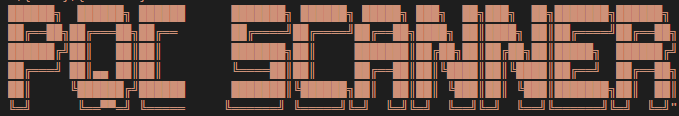
\includegraphics[width=8cm]{images/project_logo.png}

  \vspace{1cm}

  % ── Title block ───────────────────────────────────────────────────────────
  {\fontsize{32}{40}\selectfont\bfseries\color{primary} PQC CBOM Scanner}

  \vspace{0.3cm}
  {\Large\color{white!80} Cryptographic Bill of Materials}\\[0.2cm]
  {\large\color{white!60} Quantum Readiness Assessment Tool}

  \vspace{1.2cm}
  {\color{primary}\rule{0.6\textwidth}{1.5pt}}
  \vspace{0.8cm}

  % ── Document type ─────────────────────────────────────────────────────────
  {\LARGE\bfseries Software Requirements Specification}\\[0.3cm]
  {\large\color{white!70} IEEE Std 830-1998 Compliant}

  \vspace{1.5cm}

  % ── Metadata table ────────────────────────────────────────────────────────
  \begin{tabular}{rl}
    \textcolor{primary}{\textbf{Document Version}} & \textcolor{white}{1.0.0} \\[4pt]
    \textcolor{primary}{\textbf{Date}}             & \textcolor{white}{\DTMtoday} \\[4pt]
    \textcolor{primary}{\textbf{Status}}           & \textcolor{safe}{Final Draft} \\[4pt]
    \textcolor{primary}{\textbf{Project}}          & \textcolor{white}{quantumCheck} \\[4pt]
    \textcolor{primary}{\textbf{Hackathon}}        & \textcolor{white}{PNB Cybersecurity Hackathon 2025--26} \\[4pt]
    \textcolor{primary}{\textbf{Theme}}            & \textcolor{white}{Quantum-Proof Systems} \\
  \end{tabular}

  \vfill

  % ── Bottom rule ───────────────────────────────────────────────────────────
  {\color{primary}\rule{\textwidth}{3pt}}
  \vspace{0.3cm}

  \vspace{0.5cm}
\end{titlepage}
\pagecolor{white}
\color{black}


\pagenumbering{roman}
\tableofcontents
\newpage

\pagenumbering{arabic}
\setcounter{page}{1}

\chapter{Introduction}
\label{chap:introduction}

\section{Purpose}
\label{sec:purpose}

This Software Requirements Specification (SRS) document describes the functional and
non-functional requirements for the \textbf{PQC CBOM Scanner} — a web-based
cybersecurity assessment tool that audits public-facing servers for post-quantum
cryptography (PQC) readiness.

The document is intended for the following audiences:

\begin{itemize}[noitemsep]
  \item \textbf{Development Team} — as a binding technical specification during
        implementation and testing.
  \item \textbf{Security Evaluators} — as a baseline for verifying that the system
        correctly classifies TLS configurations against NIST PQC standards.
  \item \textbf{Hackathon Judges / Reviewers} — as a structured description of the
        project scope, design decisions, and requirements.
  \item \textbf{End Users} — as a reference for understanding system capabilities
        and expected behaviour.
\end{itemize}

\section{Scope}
\label{sec:scope}

The \textbf{PQC CBOM Scanner} (project codename: \textit{quantumCheck}) is a
full-stack cybersecurity tool that:

\begin{enumerate}[noitemsep]
  \item Establishes TLS handshakes with one or more user-supplied hostnames.
  \item Extracts a complete \textbf{Cryptographic Bill of Materials (CBOM)} from
        each TLS session, including cipher suite, key exchange mechanism,
        certificate details, and signature algorithms.
  \item Classifies each scanned asset against a four-tier quantum readiness
        framework aligned to NIST FIPS 203, 204, and 205.
  \item Generates a machine-readable JSON CBOM and a self-contained interactive
        HTML dashboard report.
  \item Optionally discovers and scans subdomains of a root domain using the
        Subfinder tool.
\end{enumerate}

The system is delivered as a \textbf{Dockerised web application} (Flask / Gunicorn)
with a dual interface: a browser-based GUI and a command-line interface.

\textbf{Out of scope:}
\begin{itemize}[noitemsep]
  \item Active exploitation or penetration testing of target hosts.
  \item Certificate Authority (CA) management or certificate issuance.
  \item Remediation automation (the tool provides guidance, not automated fixes).
  \item Support for non-TLS protocols (SSH, IPsec, etc.) in v1.0.
\end{itemize}

\section{Definitions, Acronyms, and Abbreviations}
\label{sec:definitions}

\begin{longtable}{L{3cm} L{11cm}}
  \toprule
  \textbf{Term} & \textbf{Definition} \\
  \midrule
  \endhead
  \bottomrule
  \endfoot
  %
  CBOM     & \textit{Cryptographic Bill of Materials} — a structured inventory
             of all cryptographic primitives used in a system or communication
             session. \\
  PQC      & \textit{Post-Quantum Cryptography} — cryptographic algorithms
             designed to resist attacks from quantum computers. \\
  TLS      & \textit{Transport Layer Security} — the standard protocol for
             encrypted communication over a network. \\
  NIST     & \textit{National Institute of Standards and Technology} — the US
             federal body responsible for cryptographic standards. \\
  FIPS     & \textit{Federal Information Processing Standard} — e.g.\
             FIPS~203 (ML-KEM), FIPS~204 (ML-DSA), FIPS~205 (SLH-DSA). \\
  ML-KEM   & \textit{Module-Lattice-based Key Encapsulation Mechanism}
             (Kyber) — a NIST-standardised PQC key exchange algorithm. \\
  ML-DSA   & \textit{Module-Lattice-based Digital Signature Algorithm}
             (Dilithium) — a NIST-standardised PQC signature scheme. \\
  SLH-DSA  & \textit{Stateless Hash-Based Digital Signature Algorithm}
             (SPHINCS+) — a NIST-standardised PQC signature scheme. \\
  FN-DSA   & \textit{Falcon Digital Signature Algorithm} — another NIST
             PQC signature standard. \\
  ECDSA    & \textit{Elliptic Curve Digital Signature Algorithm}. \\
  ECDH     & \textit{Elliptic Curve Diffie-Hellman} key exchange. \\
  RSA      & \textit{Rivest–Shamir–Adleman} public-key cryptosystem. \\
  HNDL     & \textit{Harvest Now, Decrypt Later} — a threat model where
             adversaries collect encrypted traffic today to decrypt it once
             quantum computers mature. \\
  FQS      & \textit{Fully Quantum Safe} — highest readiness tier. \\
  SSE      & \textit{Server-Sent Events} — a web API for streaming data from
             server to client. \\
  GUI      & \textit{Graphical User Interface}. \\
  CLI      & \textit{Command-Line Interface}. \\
  WSGI     & \textit{Web Server Gateway Interface} — Python web server standard. \\
  SRS      & \textit{Software Requirements Specification}. \\
\end{longtable}

\section{References}
\label{sec:references}

\begin{enumerate}[noitemsep, label={[\arabic*]}]
  \item NIST FIPS 203 — \textit{Module-Lattice-Based Key-Encapsulation Mechanism
        Standard (ML-KEM)}, August 2024.
  \item NIST FIPS 204 — \textit{Module-Lattice-Based Digital Signature Standard
        (ML-DSA)}, August 2024.
  \item NIST FIPS 205 — \textit{Stateless Hash-Based Digital Signature Standard
        (SLH-DSA)}, August 2024.
  \item IEEE Std 830-1998 — \textit{IEEE Recommended Practice for Software
        Requirements Specifications}.
  \item RFC 8446 — \textit{The Transport Layer Security (TLS) Protocol Version 1.3},
        IETF, 2018.
  \item OWASP Cryptographic Failures — \textit{OWASP Top 10 2021, A02}.
  \item ProjectDiscovery Subfinder — \url{https://github.com/projectdiscovery/subfinder}.
  \item NIST NCCoE Migration to Post-Quantum Cryptography Project, SP 1800-38.
\end{enumerate}

\section{Document Overview}
\label{sec:doc_overview}

The remainder of this SRS is structured as follows:

\begin{description}[noitemsep, leftmargin=2cm]
  \item[Chapter~\ref{chap:overall_desc}] provides a product overview, user classes,
        operating environment, and assumptions.
  \item[Chapter~\ref{chap:functional}] specifies all functional requirements grouped
        by system feature.
  \item[Chapter~\ref{chap:external_interfaces}] describes user, hardware, software,
        and communication interfaces.
  \item[Chapter~\ref{chap:nonfunctional}] defines non-functional requirements
        (performance, security, reliability, portability).
  \item[Chapter~\ref{chap:architecture}] presents the system architecture, data
        flow, and deployment model.
  \item[Chapter~\ref{chap:constraints}] lists design constraints, legal
        considerations, and dependencies.
  \item[Chapter~\ref{chap:appendix}] contains the CBOM JSON schema, quantum
        classification logic table, and version history.
\end{description}

\chapter{Overall Description}
\label{chap:overall_desc}

\section{Product Perspective}
\label{sec:product_perspective}

The PQC CBOM Scanner is a \textbf{standalone, self-contained web application} that
operates as an active TLS interrogation tool. It does not depend on any external
monitoring infrastructure, SIEM, or certificate inventory service. The system sits
entirely within a single Docker container and communicates outward only to the
user-specified target hosts.

\subsection{Context Diagram}

\begin{figure}[H]
\centering
\begin{tikzpicture}[
    sys/.style  = {rectangle, rounded corners=8pt, draw=primary, line width=1.8pt,
                   fill=sectionblue!12, text width=3cm, align=center,
                   minimum height=1.3cm, font=\small\bfseries},
    ext/.style  = {rectangle, rounded corners=5pt, draw=gray!60, line width=1pt,
                   fill=gray!8, text width=2.6cm, align=center,
                   minimum height=1.1cm, font=\small},
    arr/.style  = {-Stealth, thick},
    rarr/.style = {Stealth-, thick},
    lbl/.style  = {font=\scriptsize\itshape, fill=white, inner sep=1pt}
  ]
  % Central system
  \node[sys] (scanner) at (0,0)
    {\textcolor{primary}{PQC CBOM}\\\textcolor{primary}{Scanner}\\{\tiny(quantumCheck)}};

  % External entities
  \node[ext] (user)     at (-5,  0)   {End User\\{\tiny Browser / CLI}};
  \node[ext] (targets)  at ( 5,  0)   {Target Hosts\\{\tiny TCP/443 (TLS)}};
  \node[ext] (subfinder)at ( 0, -3.2) {Subfinder\\{\tiny Subdomain Enum}};
  \node[ext] (internet) at ( 5, -3.2) {Public Internet\\{\tiny DNS / CT Logs}};
  \node[ext] (report)   at ( 0,  3.2) {HTML Report\\{\tiny Browser View}};

  % Arrows
  \draw[arr,  color=sectionblue] (user)      -- node[lbl,above]{scan request}      (scanner);
  \draw[arr,  color=sectionblue] (scanner)   -- node[lbl,above]{TLS handshake}      (targets);
  \draw[rarr, color=sectionblue] (scanner)   -- node[lbl,right]{terminal output}    (user);
  \draw[arr,  color=sectionblue] (scanner)   -- node[lbl,right]{enumerate domains}  (subfinder);
  \draw[arr,  color=gray!70]     (subfinder) -- node[lbl,above]{DNS/CT queries}     (internet);
  \draw[arr,  color=sectionblue] (scanner)   -- node[lbl,right]{generate}           (report);
  \draw[arr,  color=sectionblue] (report)    -- node[lbl,right]{view}               (user);
\end{tikzpicture}
\caption{System Context Diagram — PQC CBOM Scanner and its external entities}
\label{fig:context_diagram}
\end{figure}

\noindent The system interacts with three external entities:

\begin{enumerate}[noitemsep]
  \item \textbf{End User} — accesses the web GUI via a browser or invokes the
        CLI scanner directly.
  \item \textbf{Target Hosts} — public-facing web servers whose TLS configuration
        is assessed. The scanner initiates outbound connections on TCP port~443
        (or user-specified ports).
  \item \textbf{Subfinder Service} — an optional embedded binary that performs
        passive and active subdomain enumeration by querying public DNS and
        certificate transparency logs.
\end{enumerate}

\subsection{Relationship to Existing Systems}

The tool is positioned as a \textit{pre-migration assessment utility} in a broader
PQC migration workflow:

\begin{center}
\resizebox{\textwidth}{!}{%
\begin{tikzpicture}[
    node distance = 0.4cm and 1.0cm,
    box/.style = {rectangle, rounded corners=4pt, draw=sectionblue,
                  fill=sectionblue!10, text width=2.4cm, align=center,
                  minimum height=1.0cm, font=\small},
    arrow/.style = {-Stealth, thick, color=primary}
  ]
  \node[box] (inv)   {Asset\\Inventory};
  \node[box, right=of inv]  (scan) {\textbf{PQC CBOM\\Scanner}};
  \node[box, right=of scan] (plan) {Migration\\Planning};
  \node[box, right=of plan] (impl) {PQC\\Implementation};
  \node[box, right=of impl] (mon)  {Continuous\\Monitoring};

  \draw[arrow] (inv)  -- (scan);
  \draw[arrow] (scan) -- (plan);
  \draw[arrow] (plan) -- (impl);
  \draw[arrow] (impl) -- (mon);
  \draw[arrow, dashed, bend right=25] (mon.south) to node[below,font=\tiny]{re-scan} (scan.south);
\end{tikzpicture}%
}
\end{center}

\section{Product Functions}
\label{sec:product_functions}

At a high level, the PQC CBOM Scanner provides the following functions:

\begin{table}[H]
  \centering
  \caption{High-Level Product Functions}
  \label{tab:product_functions}
  \begin{tabularx}{\textwidth}{C{0.5cm} L{4cm} L{9.5cm}}
    \toprule
    \textbf{\#} & \textbf{Function} & \textbf{Description} \\
    \midrule
    F1 & TLS Scanning        & Establish TLS handshakes and extract cipher,
                               key exchange, and certificate metadata. \\
    F2 & Subdomain Discovery & Enumerate subdomains of a root domain and
                               include them in the scan scope. \\
    F3 & Quantum Assessment  & Classify each asset against a four-tier PQC
                               readiness framework. \\
    F4 & CBOM Generation     & Produce a structured JSON Cryptographic Bill
                               of Materials. \\
    F5 & HTML Report         & Render a self-contained interactive HTML
                               dashboard summarising findings. \\
    F6 & Web GUI             & Provide a browser-based interface for scan
                               configuration, execution, and result viewing. \\
    F7 & Scan Control        & Allow users to start and stop scans in real time. \\
    \bottomrule
  \end{tabularx}
\end{table}

\section{User Classes and Characteristics}
\label{sec:user_classes}

\begin{table}[H]
  \centering
  \caption{User Classes}
  \label{tab:user_classes}
  \begin{tabularx}{\textwidth}{L{2.8cm} L{3.5cm} L{8cm}}
    \toprule
    \textbf{User Class} & \textbf{Technical Level} & \textbf{Primary Use Case} \\
    \midrule
    Security Analyst    & High   & Perform bulk TLS audits, interpret CBOM
                                   JSON output, integrate into workflows. \\
    System Administrator & Medium & Identify vulnerable servers before
                                   compliance deadlines; use Web GUI. \\
    CISO / Security Manager & Low & Review HTML dashboard to gauge
                                   organisation-wide quantum readiness. \\
    Developer / DevOps  & Medium & Run CLI scanner as part of CI/CD pipelines
                                   or infrastructure testing. \\
    Hackathon Evaluator & Varies & Assess tool correctness, UX, and alignment
                                   to NIST standards. \\
    \bottomrule
  \end{tabularx}
\end{table}

\section{Operating Environment}
\label{sec:operating_env}

\begin{table}[H]
  \centering
  \caption{Operating Environment}
  \label{tab:operating_env}
  \begin{tabularx}{\textwidth}{L{3.5cm} L{10cm}}
    \toprule
    \textbf{Component}       & \textbf{Requirement} \\
    \midrule
    Host OS                  & Any OS capable of running Docker (Linux,
                               macOS, Windows with WSL2). \\
    Container Runtime        & Docker Engine $\geq$ 20.10 or compatible
                               OCI runtime. \\
    Python Version           & Python 3.11 (within container). \\
    Shell Environment        & Bash 5.x (within container). \\
    OpenSSL Version          & OpenSSL $\geq$ 3.0 (within container). \\
    Network Access           & Outbound TCP/443 (or custom port) to target
                               hosts from the container. \\
    Browser (Web GUI)        & Any modern browser (Chrome $\geq$~90,
                               Firefox $\geq$~88, Edge $\geq$~90). \\
    Display Resolution       & $\geq$ 1280\texttimes720 recommended for
                               optimal dashboard layout. \\
    \bottomrule
  \end{tabularx}
\end{table}

\section{Design and Implementation Constraints}
\label{sec:design_constraints}

\begin{itemize}[noitemsep]
  \item The scanner relies on \texttt{openssl s\_client} and therefore inherits
        its support matrix for TLS extensions and PQC algorithms. OpenSSL
        versions below 3.5 may not report ML-KEM key exchange natively.
  \item The web server uses a \textbf{single Gunicorn worker} to ensure that
        in-memory scan and report state is consistent across concurrent requests.
  \item Long-running scans may exceed browser SSE connection timeouts; a 2-hour
        hard deadline is enforced server-side.
  \item Subdomain discovery requires the embedded Subfinder binary
        (\texttt{bin/subfinder}); if absent, subdomain discovery is silently
        skipped.
  \item The system does not persist data to disk beyond the \texttt{output/}
        directory; there is no database backend.
\end{itemize}

\section{Assumptions and Dependencies}
\label{sec:assumptions}

\begin{itemize}[noitemsep]
  \item Target hosts are reachable via the network from the Docker container.
  \item Target hosts use TCP port~443 by default (overridable via
        \texttt{host:port} syntax).
  \item The OpenSSL binary included in the container supports TLS~1.3.
  \item The Subfinder binary bundled in the image is version 2.13.0
        (Linux x86\_64); alternative architectures require rebuilding the image.
  \item The user has basic familiarity with web browsers and network hostnames.
  \item The tool assumes good-faith use; it does not implement rate limiting
        or access control beyond OS-level process permissions.
\end{itemize}

\chapter{Functional Requirements}
\label{chap:functional}

Requirements are identified with the prefix \textbf{FR-} (Functional Requirement).
Priority levels: \textbf{M} = Must Have, \textbf{S} = Should Have,
\textbf{C} = Could Have.

% ─────────────────────────────────────────────────────────────────────────────
\section{Feature 1: Host Input and Scan Initiation}
\label{sec:fr_input}

\begin{figure}[H]
  \centering
  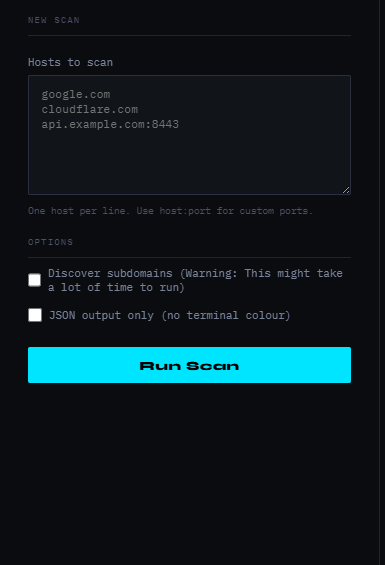
\includegraphics[width=0.55\textwidth]{images/web_input.png}
  \caption{Web GUI — Input panel with host list and scan options}
  \label{fig:gui_input}
\end{figure}

\begin{reqbox}{FR-1.1 — Multi-Host Input}
  The system \textbf{shall} accept one or more hostnames or IP addresses from the
  user, one per line, supporting the optional \texttt{host:port} syntax to override
  the default port of~443. \hfill \textbf{[M]}
\end{reqbox}

\begin{reqbox}{FR-1.2 — File-Based Input (CLI)}
  The CLI scanner \textbf{shall} accept a plain-text file of hosts via the
  \texttt{-f \textless{}file\textgreater{}} flag, skipping blank lines and lines
  beginning with \texttt{\#}. \hfill \textbf{[M]}
\end{reqbox}

\begin{reqbox}{FR-1.3 — Scan Configuration Options}
  The Web GUI \textbf{shall} expose at minimum the following boolean options
  prior to scan start:
  \begin{itemize}[noitemsep]
    \item \textbf{Discover Subdomains} — invoke Subfinder before scanning.
    \item \textbf{JSON Output Only} — suppress ANSI colour codes in terminal
          output.
  \end{itemize}
  \hfill \textbf{[M]}
\end{reqbox}

\begin{reqbox}{FR-1.4 — Scan Button State Management}
  The \textit{Run Scan} button \textbf{shall} be disabled while a scan is in
  progress and re-enabled upon completion or cancellation to prevent duplicate
  scans. \hfill \textbf{[M]}
\end{reqbox}

% ─────────────────────────────────────────────────────────────────────────────
\section{Feature 2: TLS Scanning Engine}
\label{sec:fr_tls}

\begin{reqbox}{FR-2.1 — TLS Handshake Initiation}
  For each host in the scan list, the system \textbf{shall} initiate a TLS~1.3
  handshake using \texttt{openssl s\_client} with a per-host timeout of 8 seconds.
  \hfill \textbf{[M]}
\end{reqbox}

\begin{reqbox}{FR-2.2 — TLS Version Extraction}
  The system \textbf{shall} extract and record the negotiated TLS protocol version
  (TLS~1.0, 1.1, 1.2, or 1.3). \hfill \textbf{[M]}
\end{reqbox}

\begin{reqbox}{FR-2.3 — Cipher Suite Extraction}
  The system \textbf{shall} extract the negotiated cipher suite name (e.g.\
  \texttt{TLS\_AES\_256\_GCM\_SHA384}). \hfill \textbf{[M]}
\end{reqbox}

\begin{reqbox}{FR-2.4 — Key Exchange Extraction}
  The system \textbf{shall} extract the key exchange algorithm from the TLS
  handshake, including hybrid PQC variants (e.g.\ \texttt{X25519Kyber768},
  \texttt{ML-KEM-768}). \hfill \textbf{[M]}
\end{reqbox}

\begin{reqbox}{FR-2.5 — Certificate Chain Extraction}
  The system \textbf{shall} extract the following fields from the server's leaf
  certificate:
  \begin{itemize}[noitemsep]
    \item Subject Distinguished Name
    \item Issuer Distinguished Name
    \item Public key algorithm and bit-length
    \item Signature algorithm
    \item Validity period (not-before, not-after)
    \item Certificate chain depth
  \end{itemize}
  \hfill \textbf{[M]}
\end{reqbox}

\begin{reqbox}{FR-2.6 — Connection Failure Handling}
  If the TLS handshake fails (timeout, refused, unreachable), the system
  \textbf{shall} record a \texttt{connection\_error} entry in the CBOM for that
  host rather than aborting the entire scan. \hfill \textbf{[M]}
\end{reqbox}

\begin{reqbox}{FR-2.7 — Certificate Verification Status}
  The system \textbf{shall} record whether the server certificate chain
  verification succeeded or failed during the handshake. \hfill \textbf{[S]}
\end{reqbox}

% ─────────────────────────────────────────────────────────────────────────────
\section{Feature 3: Quantum Readiness Classification}
\label{sec:fr_classification}

\subsection{Classification Tiers}
\label{subsec:tiers}

\begin{table}[H]
  \centering
  \caption{Quantum Readiness Tiers}
  \label{tab:tiers}
  \begin{tabularx}{\textwidth}{C{0.4cm} L{3.5cm} L{4.2cm} L{5.5cm}}
    \toprule
    \textbf{\#} & \textbf{Label} & \textbf{Symbol} & \textbf{Criteria} \\
    \midrule
    1 & Fully Quantum Safe & \textcolor{safe}{\textbf{\fqssym{} FQS}} &
        PQC key exchange \textit{and} ML-DSA/SLH-DSA/FN-DSA certificate
        \textit{and} AES-256 or ChaCha20 symmetric cipher. \\
    \addlinespace
    2 & PQC Ready & \textcolor{pqcready}{\textbf{\pqcsym{} PQC}} &
        PQC key exchange \textit{and} safe symmetric cipher, but
        classical (RSA/ECDSA) certificate. \\
    \addlinespace
    3 & Not PQC Ready & \textcolor{notpqc}{\textbf{\notpqcsym{} NOT}} &
        Classical key exchange (X25519, ECDH, RSA-KEM) \textit{or}
        AES-128 symmetric cipher (marginal security). \\
    \addlinespace
    4 & Critical & \textcolor{critical}{\textbf{\critsym{} CRIT}} &
        Broken symmetric cipher: 3DES, RC4, DES, or export-grade. \\
    \bottomrule
  \end{tabularx}
\end{table}

\begin{reqbox}{FR-3.1 — Key Exchange Classification}
  The system \textbf{shall} classify the key exchange as:
  \begin{itemize}[noitemsep]
    \item \texttt{pqc\_hybrid} — X25519Kyber768 or similar hybrid.
    \item \texttt{pqc\_pure} — pure ML-KEM or equivalent.
    \item \texttt{classical} — X25519, ECDH, secp256r1, RSA, etc.
    \item \texttt{unknown} — could not be determined from handshake output.
  \end{itemize}
  \hfill \textbf{[M]}
\end{reqbox}

\begin{reqbox}{FR-3.2 — Certificate Classification}
  The system \textbf{shall} classify the server certificate algorithm as:
  \begin{itemize}[noitemsep]
    \item \texttt{pqc} — ML-DSA, SLH-DSA, FN-DSA (Falcon).
    \item \texttt{ecdsa} — EC-based signature.
    \item \texttt{rsa} — RSA-based signature.
    \item \texttt{unknown} — unrecognised algorithm.
  \end{itemize}
  \hfill \textbf{[M]}
\end{reqbox}

\begin{reqbox}{FR-3.3 — Symmetric Cipher Classification}
  The system \textbf{shall} classify the negotiated symmetric cipher as:
  \begin{itemize}[noitemsep]
    \item \texttt{safe} — AES-256-GCM, ChaCha20-Poly1305.
    \item \texttt{marginal} — AES-128-GCM (weakened to 64-bit by Grover's
          algorithm against a quantum adversary).
    \item \texttt{broken} — 3DES, RC4, DES, NULL, EXPORT ciphers.
    \item \texttt{unknown} — unrecognised cipher suite.
  \end{itemize}
  \hfill \textbf{[M]}
\end{reqbox}

\begin{reqbox}{FR-3.4 — Composite Quantum Label Assignment}
  The system \textbf{shall} assign one of the four tiers defined in
  Table~\ref{tab:tiers} to each scanned host based on the combination of
  key exchange, certificate, and symmetric cipher classifications. \hfill \textbf{[M]}
\end{reqbox}

\begin{reqbox}{FR-3.5 — Vulnerability List Generation}
  For each host, the system \textbf{shall} generate a human-readable list of
  specific vulnerabilities identified, including:
  \begin{itemize}[noitemsep]
    \item Key exchange susceptibility to Shor's algorithm.
    \item RSA/ECDSA certificate susceptibility to Shor's algorithm.
    \item AES-128 bit-security reduction by Grover's algorithm.
    \item Broken cipher suites (3DES, RC4, etc.).
    \item Certificate expiry (expired or $<$~30 days remaining).
  \end{itemize}
  \hfill \textbf{[M]}
\end{reqbox}

\begin{reqbox}{FR-3.6 — Actionable Recommendations}
  The system \textbf{shall} generate context-aware, label-specific remediation
  recommendations for each host, referencing concrete migration steps
  (e.g.\ enabling X25519Kyber768, upgrading to ML-DSA certificate,
  disabling 3DES). \hfill \textbf{[M]}
\end{reqbox}

% ─────────────────────────────────────────────────────────────────────────────
\section{Feature 4: Subdomain Discovery}
\label{sec:fr_subdomain}

\begin{reqbox}{FR-4.1 — Subfinder Integration}
  When the \textit{Discover Subdomains} option is enabled and the Subfinder
  binary is present, the system \textbf{shall} execute Subfinder against the
  root domain of each supplied host with a 120-second timeout. \hfill \textbf{[S]}
\end{reqbox}

\begin{reqbox}{FR-4.2 — Subdomain Merging}
  Discovered subdomains \textbf{shall} be merged into the scan host list and
  scanned with the same TLS pipeline as explicit hosts. \hfill \textbf{[S]}
\end{reqbox}

\begin{reqbox}{FR-4.3 — Graceful Degradation}
  If Subfinder is not available, the system \textbf{shall} silently skip
  subdomain discovery and proceed with only the user-supplied hosts.
  \hfill \textbf{[M]}
\end{reqbox}

% ─────────────────────────────────────────────────────────────────────────────
\section{Feature 5: CBOM JSON Output}
\label{sec:fr_cbom}

\begin{reqbox}{FR-5.1 — Machine-Readable CBOM}
  The system \textbf{shall} produce a JSON CBOM document conforming to the schema
  defined in Appendix~\ref{sec:cbom_schema}. \hfill \textbf{[M]}
\end{reqbox}

\begin{reqbox}{FR-5.2 — CBOM Metadata}
  The CBOM \textbf{shall} include top-level metadata: scan start timestamp,
  scan end timestamp, and total host count. \hfill \textbf{[M]}
\end{reqbox}

\begin{reqbox}{FR-5.3 — Per-Asset CBOM Entry}
  Each scanned host \textbf{shall} produce a CBOM asset entry containing at
  minimum: hostname, port, TLS version, cipher suite, key exchange (type and
  algorithm), certificate details, symmetric cipher, quantum label, vulnerability
  list, recommendations, and scan timestamp. \hfill \textbf{[M]}
\end{reqbox}

\begin{reqbox}{FR-5.4 — JSON File Persistence}
  The system \textbf{shall} write the final CBOM JSON to the \texttt{output/}
  directory with a timestamp-based filename. \hfill \textbf{[S]}
\end{reqbox}

% ─────────────────────────────────────────────────────────────────────────────
\section{Feature 6: Interactive HTML Report}
\label{sec:fr_report}

\begin{figure}[H]
  \centering
  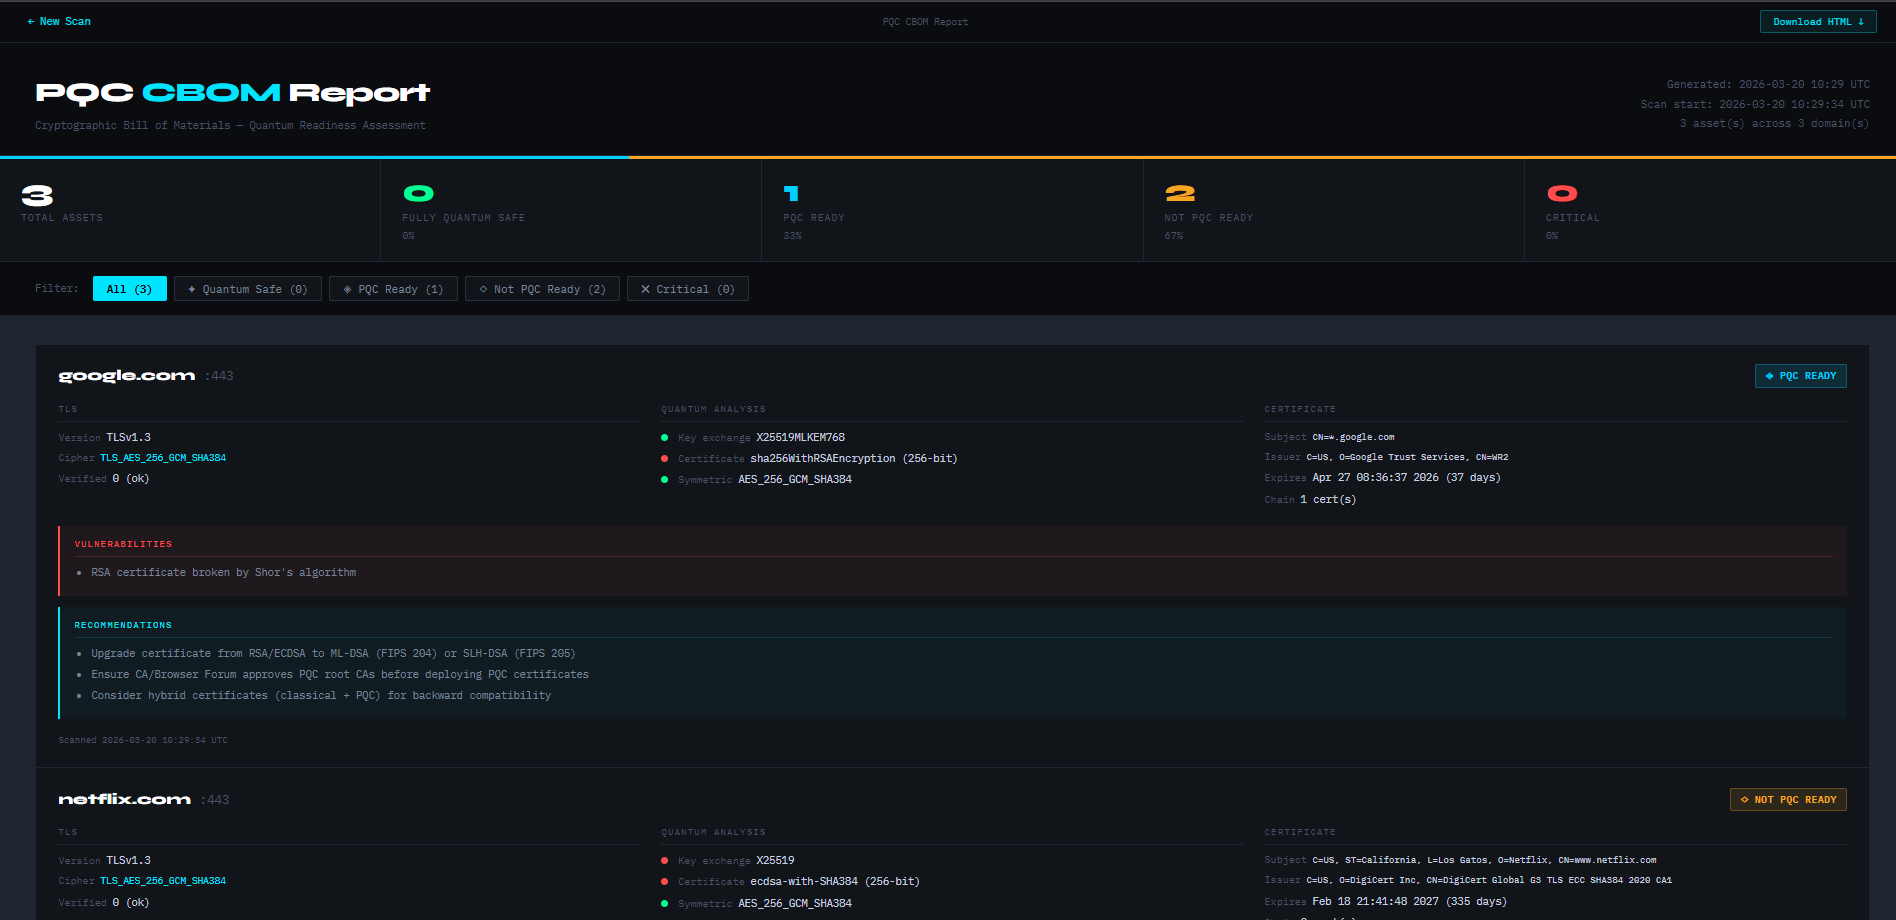
\includegraphics[width=\textwidth]{images/html_report.png}
  \caption{HTML Report — Stats bar, progress bar, and asset cards}
  \label{fig:html_report_overview}
\end{figure}

\begin{reqbox}{FR-6.1 — Self-Contained HTML}
  The generated report \textbf{shall} be a single self-contained HTML file with
  all CSS and JavaScript embedded inline, requiring no internet connection to
  render. \hfill \textbf{[M]}
\end{reqbox}

\begin{reqbox}{FR-6.2 — Summary Statistics}
  The report header \textbf{shall} display total asset count and per-tier count
  with percentage for each of the four quantum readiness labels. \hfill \textbf{[M]}
\end{reqbox}

\begin{reqbox}{FR-6.3 — Visual Progress Bar}
  The report \textbf{shall} render a horizontal progress bar with colour-coded
  segments proportional to the count of each tier, providing an at-a-glance
  portfolio health view. \hfill \textbf{[M]}
\end{reqbox}

\begin{reqbox}{FR-6.4 — Filter Controls}
  The report \textbf{shall} provide interactive filter buttons to show only assets
  matching a selected tier label (All / FQS / PQC / Not PQC / Critical) without
  a page reload. \hfill \textbf{[M]}
\end{reqbox}

\begin{reqbox}{FR-6.5 — Domain Grouping}
  Assets \textbf{shall} be grouped by their root domain (eTLD+1), with subdomains
  displayed in a collapsible drawer beneath the root asset card. \hfill \textbf{[S]}
\end{reqbox}

\begin{reqbox}{FR-6.6 — Asset Card Detail}
  Each asset card \textbf{shall} display:
  \begin{itemize}[noitemsep]
    \item TLS version and cipher suite.
    \item Key exchange algorithm and PQC classification dot.
    \item Certificate subject, issuer, expiry (colour-coded), and chain depth.
    \item Signature algorithm and PQC classification dot.
    \item Symmetric cipher and safety dot.
    \item Vulnerability list.
    \item Recommendation list.
    \item Scan timestamp.
  \end{itemize}
  \hfill \textbf{[M]}
\end{reqbox}

\begin{reqbox}{FR-6.7 — Certificate Expiry Warnings}
  Certificate expiry \textbf{shall} be displayed in:
  \begin{itemize}[noitemsep]
    \item \textcolor{critical}{\textbf{Red}} — certificate already expired.
    \item \textcolor{notpqc}{\textbf{Amber}} — fewer than 30 days remaining.
    \item Normal colour — otherwise.
  \end{itemize}
  \hfill \textbf{[M]}
\end{reqbox}

\begin{reqbox}{FR-6.8 — Report Download}
  The report page \textbf{shall} provide a \textit{Download HTML} button that
  saves the report as a standalone file to the user's local machine. \hfill \textbf{[S]}
\end{reqbox}

% ─────────────────────────────────────────────────────────────────────────────
\section{Feature 7: Web GUI and Real-Time Streaming}
\label{sec:fr_gui}

\begin{figure}[H]
  \centering
  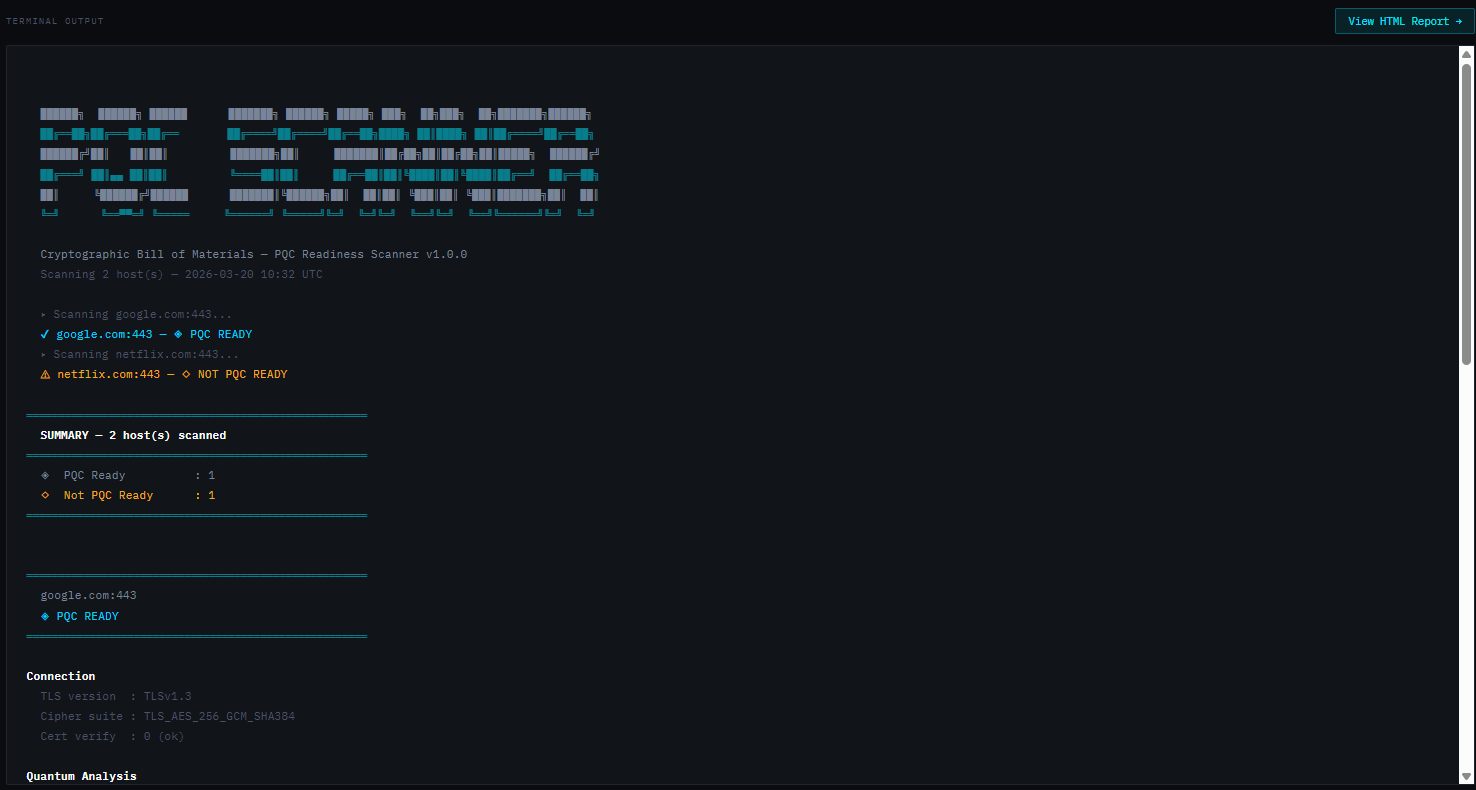
\includegraphics[width=\textwidth]{images/web_terminal_output.png}
  \caption{Web GUI — Terminal output panel with real-time SSE streaming}
  \label{fig:gui_terminal}
\end{figure}

\begin{reqbox}{FR-7.1 — Real-Time Output Streaming}
  The web application \textbf{shall} stream scan output to the browser in real time
  using Server-Sent Events (SSE), rendering each line as it is produced by the
  scanner. \hfill \textbf{[M]}
\end{reqbox}

\begin{reqbox}{FR-7.2 — ANSI Colour Rendering}
  Colour codes emitted by the scanner (\texttt{\\033[...m} sequences)
  \textbf{shall} be converted to appropriate HTML/CSS styling so that tier labels
  appear in their corresponding colours in the browser output panel. \hfill \textbf{[M]}
\end{reqbox}

\begin{reqbox}{FR-7.3 — Scan Status Indicator}
  A spinner or progress indicator \textbf{shall} be visible while a scan is
  running and hidden upon completion. \hfill \textbf{[S]}
\end{reqbox}

\begin{reqbox}{FR-7.4 — Report Link Post-Scan}
  Upon successful scan completion, the GUI \textbf{shall} display a
  \textit{View HTML Report} link that opens the generated report in a new
  browser tab. \hfill \textbf{[M]}
\end{reqbox}

\begin{reqbox}{FR-7.5 — Stop Scan}
  The GUI \textbf{shall} provide a \textit{Stop Scan} button that becomes visible
  during a running scan and, when clicked, sends a SIGTERM to the scanner
  process to terminate it gracefully. \hfill \textbf{[M]}
\end{reqbox}

\begin{reqbox}{FR-7.6 — SSE Keepalive}
  The SSE stream \textbf{shall} emit a keepalive comment every 5 seconds to
  prevent intermediate proxies from closing the connection prematurely.
  \hfill \textbf{[S]}
\end{reqbox}

% ─────────────────────────────────────────────────────────────────────────────
\section{Feature 8: Report Lifecycle Management}
\label{sec:fr_lifecycle}

\begin{reqbox}{FR-8.1 — In-Memory Report Storage}
  Generated reports \textbf{shall} be held in server memory and accessible via a
  unique report identifier for the duration of the configured TTL (default:
  3600 seconds). \hfill \textbf{[M]}
\end{reqbox}

\begin{reqbox}{FR-8.2 — Automatic Report Eviction}
  A background daemon thread \textbf{shall} evict expired reports every 5 minutes
  to prevent unbounded memory growth. \hfill \textbf{[M]}
\end{reqbox}

\begin{reqbox}{FR-8.3 — TTL Configuration}
  The report TTL \textbf{shall} be configurable via the \texttt{REPORT\_TTL}
  environment variable without code changes. \hfill \textbf{[S]}
\end{reqbox}

\chapter{External Interface Requirements}
\label{chap:external_interfaces}

\section{User Interfaces}
\label{sec:ui}

\subsection{Web GUI}

The primary user interface is a single-page web application served at
\texttt{http://localhost:5000} (or the configured \texttt{PORT}).

\subsubsection{Layout Overview}

\begin{figure}[H]
  \centering
  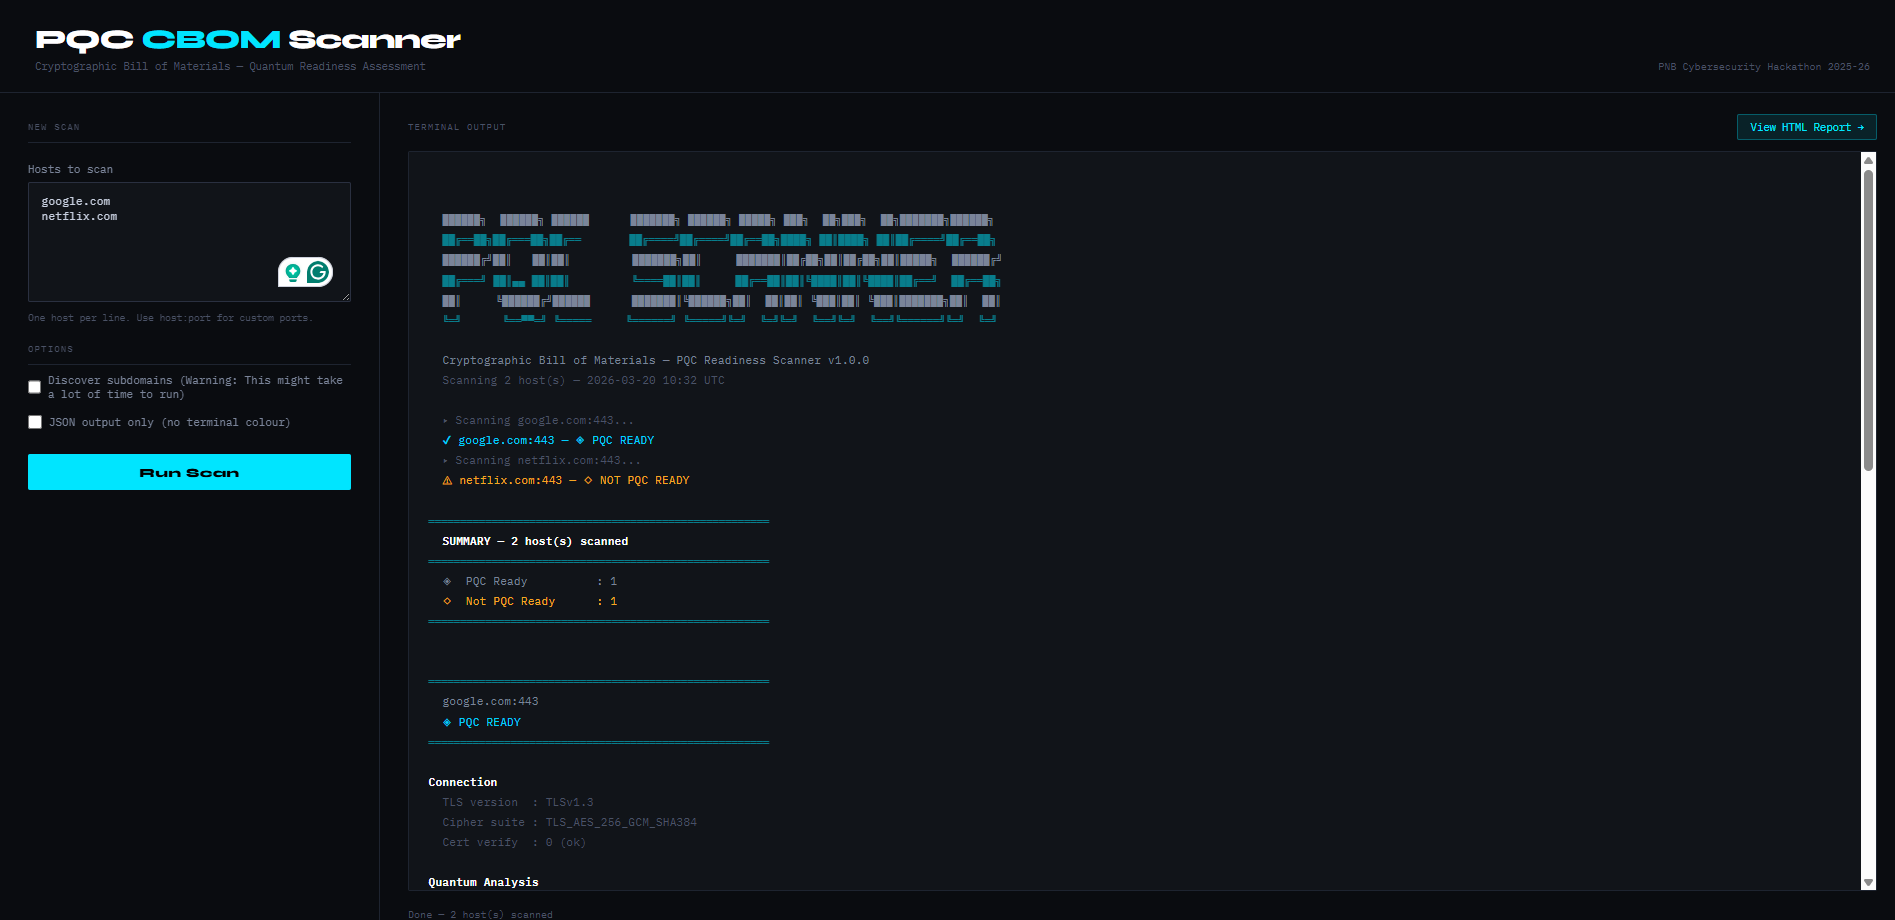
\includegraphics[width=\textwidth]{images/web_gui_full_output.png}
  \caption{Web GUI — Full layout: header, input panel (left), and output panel (right)}
  \label{fig:gui_full_layout}
\end{figure}

\noindent The page is divided into three regions:

\begin{description}[noitemsep, leftmargin=2cm]
  \item[Header] Application title (\textit{PQC CBOM Scanner}) with a cyan accent
    on \textit{CBOM}, subtitle, and hackathon context badge.
  \item[Left Panel (Input)] Host textarea, option checkboxes, Run Scan and Stop Scan
    buttons, version info footer.
  \item[Right Panel (Output)] Terminal-style scrollable output area with real-time
    SSE content, scan status spinner, and post-scan report link.
\end{description}

\subsubsection{Colour Scheme}

\begin{table}[H]
  \centering
  \caption{UI Colour Conventions}
  \label{tab:ui_colours}
  \begin{tabular}{L{4cm} L{3cm} L{7cm}}
    \toprule
    \textbf{Element} & \textbf{Hex Value} & \textbf{Usage} \\
    \midrule
    Background       & \texttt{\#0A0C10}  & Page and panel backgrounds. \\
    Cyan Accent      & \texttt{\#00E5FF}  & Headings, buttons, borders. \\
    Fully Quantum Safe & \texttt{\#00FF94} & FQS label, dots, text. \\
    PQC Ready        & \texttt{\#00BFFF}  & PQC label, dots, text. \\
    Not PQC Ready    & \texttt{\#F5A623}  & NOT label, warnings, dots. \\
    Critical         & \texttt{\#FF4D4D}  & CRIT label, errors, stop button. \\
    \bottomrule
  \end{tabular}
\end{table}

\subsubsection{Typography}

\begin{itemize}[noitemsep]
  \item \textbf{Syne} (Google Fonts) — used for headings and labels.
  \item \textbf{IBM Plex Mono} (Google Fonts) — used for monospace terminal
        output, code, and cipher names.
\end{itemize}

\subsection{HTML Report Interface}

\begin{figure}[H]
  \centering
  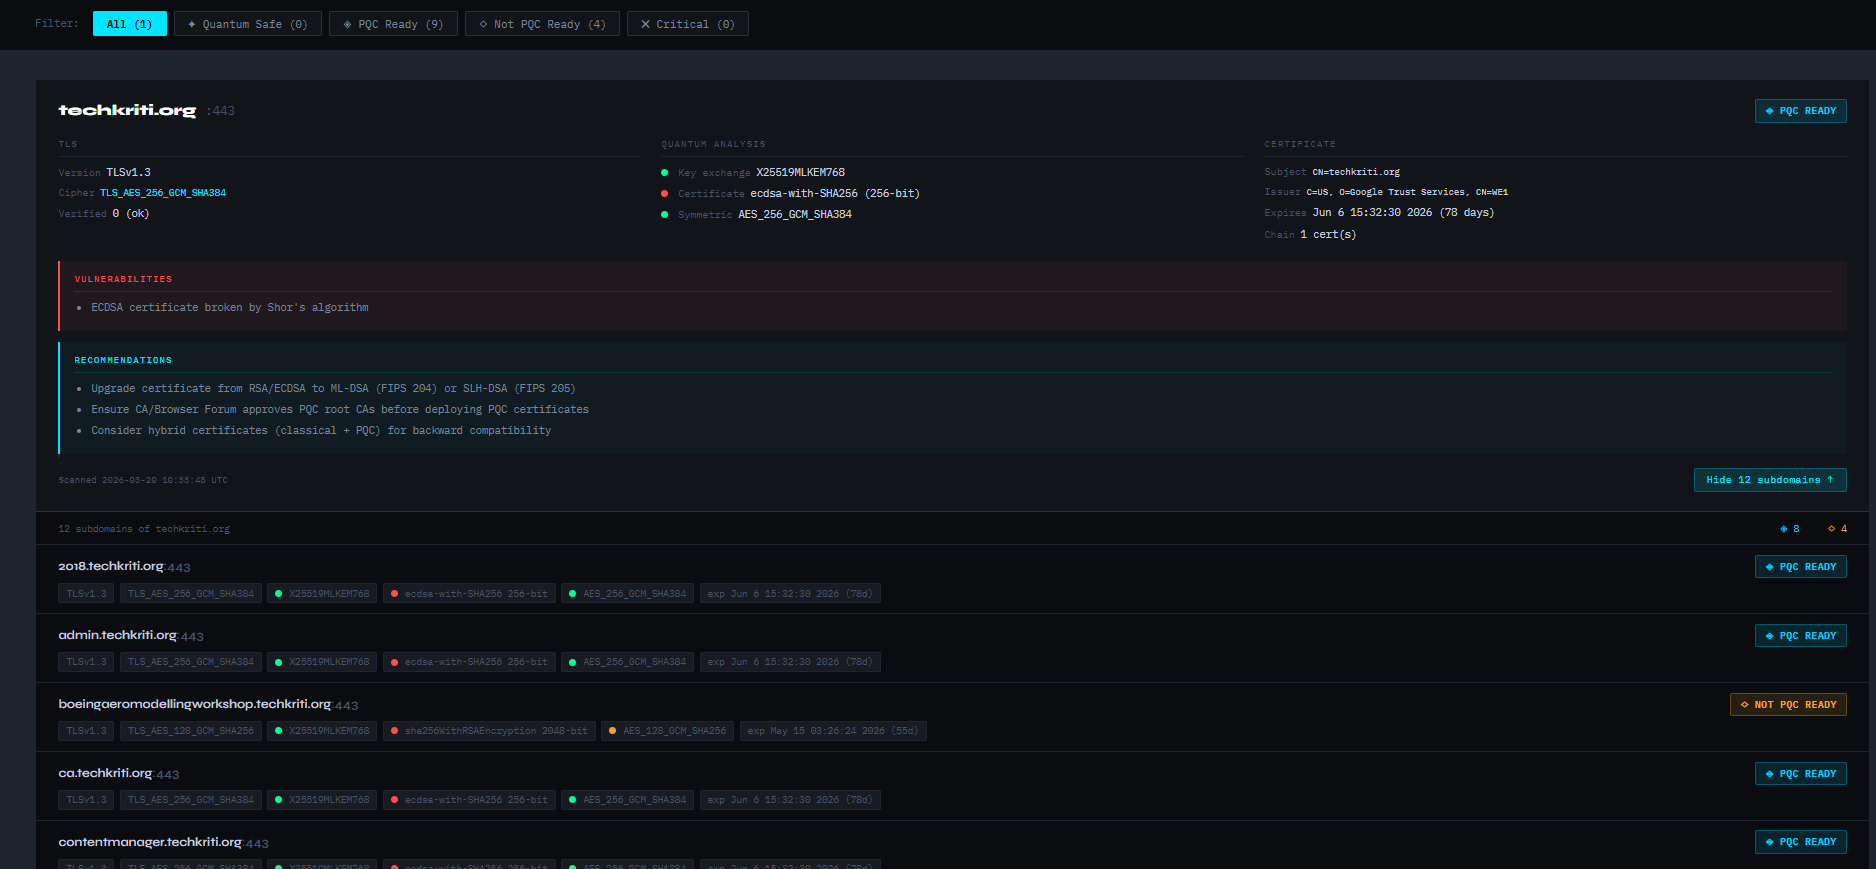
\includegraphics[width=\textwidth]{images/html_report_with_subdomain.png}
  \caption{HTML Report — Filter bar and domain group with subdomain drawer expanded}
  \label{fig:html_report_filter}
\end{figure}

The generated report provides the following interactive UI elements:

\begin{itemize}[noitemsep]
  \item \textbf{Sticky navigation bar} — Back to New Scan link and Download HTML
        button always visible while scrolling.
  \item \textbf{Statistics cells} — large numerals showing count and percentage
        per tier.
  \item \textbf{Progress bar} — colour-segmented horizontal bar.
  \item \textbf{Filter buttons} — toggle visibility of asset cards by tier.
  \item \textbf{Domain groups} — root asset card + collapsible subdomain drawer
        with compact subdomain rows.
  \item \textbf{Asset cards} — full CBOM detail per host with colour-coded
        indicator dots.
\end{itemize}

\subsection{Command-Line Interface}

The CLI scanner (\texttt{scan.sh}) accepts the following arguments:

\begin{table}[H]
  \centering
  \caption{CLI Arguments}
  \label{tab:cli_args}
  \begin{tabularx}{\textwidth}{L{3.5cm} L{10cm}}
    \toprule
    \textbf{Argument} & \textbf{Description} \\
    \midrule
    \texttt{<host>}          & One or more space-separated hostnames. \\
    \texttt{-f <file>}       & Read hosts from a plain-text file. \\
    \texttt{--subdomains}    & Enable Subfinder subdomain discovery. \\
    \texttt{--json}          & Output clean JSON; suppress ANSI codes. \\
    \texttt{--report}        & Generate an HTML report after scanning. \\
    \bottomrule
  \end{tabularx}
\end{table}

\section{Hardware Interfaces}
\label{sec:hardware_interfaces}

The application has no direct hardware interface requirements. It runs entirely
in software and communicates over standard Ethernet/Wi-Fi network interfaces via
the host OS's TCP/IP stack. No special hardware (HSM, SmartCard, etc.) is
required.

\section{Software Interfaces}
\label{sec:software_interfaces}

\begin{table}[H]
  \centering
  \caption{Software Interface Dependencies}
  \label{tab:software_interfaces}
  \begin{tabularx}{\textwidth}{L{3cm} L{2.5cm} L{8.5cm}}
    \toprule
    \textbf{Component} & \textbf{Version} & \textbf{Role} \\
    \midrule
    Python             & 3.11             & Application runtime. \\
    Flask              & $\geq$ 3.0       & HTTP framework; routes, SSE, template rendering. \\
    Gunicorn           & $\geq$ 21.0      & Production WSGI server (gthread worker). \\
    OpenSSL            & $\geq$ 3.0       & TLS handshake and certificate parsing via
                                           \texttt{s\_client}. \\
    Bash               & 5.x              & Scanner script (\texttt{scan.sh}); host
                                           loop, JSON assembly. \\
    Subfinder          & 2.13.0           & Passive/active subdomain enumeration. \\
    Docker             & $\geq$ 20.10     & Container packaging and runtime. \\
    \bottomrule
  \end{tabularx}
\end{table}

\section{Communication Interfaces}
\label{sec:communication_interfaces}

\begin{table}[H]
  \centering
  \caption{Communication Interfaces}
  \label{tab:comm_interfaces}
  \begin{tabularx}{\textwidth}{L{3.5cm} L{2.5cm} L{8cm}}
    \toprule
    \textbf{Interface} & \textbf{Protocol} & \textbf{Description} \\
    \midrule
    Browser $\leftrightarrow$ App & HTTP/1.1 & Form submission, page requests,
                                               report download. \\
    Browser $\leftarrow$ App (SSE) & HTTP/1.1 & Server-Sent Events stream of
                                                scan output lines. \\
    App $\rightarrow$ Target Hosts & TLS 1.3 (TCP/443) & Outbound TLS
                                                          handshake for
                                                          interrogation. \\
    App $\rightarrow$ Subfinder & STDIN/STDOUT & Local IPC pipe; domain input
                                                 and subdomain output. \\
    Subfinder $\rightarrow$ Internet & DNS / HTTPS & Queries public DNS resolvers
                                                      and certificate transparency
                                                      logs. \\
    \bottomrule
  \end{tabularx}
\end{table}

\noindent\textbf{Port assignments:}
\begin{itemize}[noitemsep]
  \item \texttt{5000/TCP} — Web GUI HTTP server (configurable via \texttt{PORT}
        env var).
  \item \texttt{443/TCP} — Default outbound port for TLS target connections
        (overridable per host).
\end{itemize}

\chapter{Non-Functional Requirements}
\label{chap:nonfunctional}

Non-functional requirements are identified with the prefix \textbf{NFR-}.

% ─────────────────────────────────────────────────────────────────────────────
\section{Performance Requirements}
\label{sec:perf}

\begin{reqbox}{NFR-P.1 — Per-Host Scan Timeout}
  Each TLS handshake attempt \textbf{shall} complete or time out within
  \textbf{8 seconds}, ensuring predictable throughput when scanning large host
  lists. \hfill \textbf{[M]}
\end{reqbox}

\begin{reqbox}{NFR-P.2 — Subdomain Discovery Timeout}
  Subfinder execution per root domain \textbf{shall} be capped at
  \textbf{120 seconds} to prevent the overall scan from hanging indefinitely.
  \hfill \textbf{[M]}
\end{reqbox}

\begin{reqbox}{NFR-P.3 — SSE Stream Hard Deadline}
  Each Server-Sent Events stream \textbf{shall} be terminated after a maximum
  of \textbf{2 hours} server-side to prevent resource leaks from abandoned
  browser connections. \hfill \textbf{[M]}
\end{reqbox}

\begin{reqbox}{NFR-P.4 — Concurrent Request Capacity}
  The Gunicorn configuration with \textbf{1 worker and 16 threads}
  \textbf{shall} support at least 8 simultaneous SSE connections and
  associated background scan jobs without degradation. \hfill \textbf{[S]}
\end{reqbox}

\begin{reqbox}{NFR-P.5 — Report Generation Latency}
  HTML report generation from a complete CBOM JSON \textbf{shall} complete
  within \textbf{5 seconds} for scan results containing up to 500 hosts.
  \hfill \textbf{[S]}
\end{reqbox}

\begin{reqbox}{NFR-P.6 — UI Responsiveness}
  The web GUI \textbf{shall} remain responsive (non-blocking user interaction)
  during active scanning; SSE streaming \textbf{shall not} freeze the browser tab.
  \hfill \textbf{[M]}
\end{reqbox}

% ─────────────────────────────────────────────────────────────────────────────
\section{Security Requirements}
\label{sec:security}

\begin{reqbox}{NFR-S.1 — No Persistent Secret Storage}
  The system \textbf{shall not} store, log, or transmit any private keys,
  session tokens, or user credentials. The application is read-only with respect
  to target host data. \hfill \textbf{[M]}
\end{reqbox}

\begin{reqbox}{NFR-S.2 — Input Sanitisation}
  Host input provided by the user \textbf{shall} be validated and sanitised
  before being passed to shell commands to prevent command injection.
  \hfill \textbf{[M]}
\end{reqbox}

\begin{reqbox}{NFR-S.3 — No Destructive Operations on Targets}
  The scanner \textbf{shall} perform only passive TLS interrogation (initiating
  a standard TLS handshake). No vulnerability exploitation, fuzzing, or denial
  of service techniques \textbf{shall} be employed. \hfill \textbf{[M]}
\end{reqbox}

\begin{reqbox}{NFR-S.4 — Container Isolation}
  When deployed via Docker, the application \textbf{shall} run as a non-root
  user inside the container to minimise the blast radius of any security
  vulnerability. \hfill \textbf{[S]}
\end{reqbox}

\begin{reqbox}{NFR-S.5 — CBOM Data Confidentiality}
  CBOM JSON files written to \texttt{output/} \textbf{shall} be readable
  only by the OS user running the container. No report \textbf{shall} be
  exposed to the public internet without explicit user action. \hfill \textbf{[S]}
\end{reqbox}

\begin{reqbox}{NFR-S.6 — XSS Prevention in Report}
  All host-derived data embedded in the HTML report \textbf{shall} be HTML-escaped
  to prevent cross-site scripting (XSS) if the report is viewed in a shared
  browser context. \hfill \textbf{[M]}
\end{reqbox}

% ─────────────────────────────────────────────────────────────────────────────
\section{Reliability and Availability}
\label{sec:reliability}

\begin{reqbox}{NFR-R.1 — Graceful Connection Failure Handling}
  A failed TLS connection to any individual host \textbf{shall not} abort the
  scan of remaining hosts; the failure \textbf{shall} be recorded in the CBOM
  and scanning \textbf{shall} continue. \hfill \textbf{[M]}
\end{reqbox}

\begin{reqbox}{NFR-R.2 — JSON Output Validity}
  The CBOM JSON produced by the scanner \textbf{shall} always be valid,
  well-formed JSON. Special characters in hostnames, certificate fields, or
  cipher names \textbf{shall} be properly escaped. \hfill \textbf{[M]}
\end{reqbox}

\begin{reqbox}{NFR-R.3 — Report Generation on Partial Failure}
  If one or more hosts in a scan produce errors, the HTML report
  \textbf{shall} still be generated for all hosts that were successfully
  scanned. \hfill \textbf{[M]}
\end{reqbox}

\begin{reqbox}{NFR-R.4 — Memory Leak Prevention}
  The background report reaper thread \textbf{shall} prevent unbounded
  accumulation of in-memory reports by evicting entries that exceed the TTL.
  \hfill \textbf{[M]}
\end{reqbox}

% ─────────────────────────────────────────────────────────────────────────────
\section{Maintainability}
\label{sec:maintainability}

\begin{reqbox}{NFR-M.1 — Modular Architecture}
  The system \textbf{shall} maintain a clear separation of concerns:
  \begin{itemize}[noitemsep]
    \item \texttt{scan.sh} — TLS scanning and CBOM JSON generation.
    \item \texttt{app.py} — Web server, SSE streaming, process management.
    \item \texttt{generate\_report.py} — HTML report rendering.
  \end{itemize}
  \hfill \textbf{[M]}
\end{reqbox}

\begin{reqbox}{NFR-M.2 — Classification Logic Isolation}
  Quantum readiness classification logic \textbf{shall} be implemented in a
  single, clearly labelled block within \texttt{scan.sh} so that updates
  to NIST standards can be applied by editing one location. \hfill \textbf{[S]}
\end{reqbox}

\begin{reqbox}{NFR-M.3 — Environment-Based Configuration}
  All tunable parameters (port, TTL, output path) \textbf{shall} be
  configurable via environment variables with sensible defaults, requiring
  no code changes for deployment customisation. \hfill \textbf{[S]}
\end{reqbox}

% ─────────────────────────────────────────────────────────────────────────────
\section{Portability}
\label{sec:portability}

\begin{reqbox}{NFR-PO.1 — Docker Portability}
  The application \textbf{shall} be fully self-contained within its Docker
  image, including all runtime dependencies (Python, Flask, OpenSSL, Bash,
  Subfinder), requiring only Docker Engine on the host. \hfill \textbf{[M]}
\end{reqbox}

\begin{reqbox}{NFR-PO.2 — Architecture Note}
  The bundled Subfinder binary targets Linux x86\_64. For ARM64 or other
  architectures, the Dockerfile \textbf{shall} be rebuilt with the appropriate
  binary. The rest of the application \textbf{shall} be architecture-agnostic.
  \hfill \textbf{[S]}
\end{reqbox}

\begin{reqbox}{NFR-PO.3 — Browser Compatibility}
  The web GUI and HTML report \textbf{shall} render correctly in all
  evergreen browsers (Chrome, Firefox, Edge, Safari) without requiring
  browser plugins or extensions. \hfill \textbf{[M]}
\end{reqbox}

% ─────────────────────────────────────────────────────────────────────────────
\section{Usability}
\label{sec:usability}

\begin{reqbox}{NFR-U.1 — Colour-Coded Tier Display}
  All four quantum readiness tiers \textbf{shall} be visually distinguished
  by consistent colour coding across the terminal output, HTML report, and
  asset cards (Table~\ref{tab:ui_colours}). \hfill \textbf{[M]}
\end{reqbox}

\begin{reqbox}{NFR-U.2 — Zero-Installation Web Access}
  A user \textbf{shall} be able to use the full Web GUI without installing any
  software beyond Docker; no Node.js, npm, or frontend build step is required.
  \hfill \textbf{[M]}
\end{reqbox}

\begin{reqbox}{NFR-U.3 — Offline Report Viewing}
  A downloaded HTML report \textbf{shall} be fully viewable offline without
  any network request. \hfill \textbf{[M]}
\end{reqbox}

\chapter{System Architecture}
\label{chap:architecture}

\section{Architectural Overview}
\label{sec:arch_overview}

The PQC CBOM Scanner follows a \textbf{three-tier architecture} within a single
Docker container:

\begin{enumerate}[noitemsep]
  \item \textbf{Presentation Tier} — Flask-served HTML/JS/CSS web GUI and
        generated HTML report.
  \item \textbf{Application Tier} — Flask application (\texttt{app.py}) managing
        scan orchestration, SSE streaming, process lifecycle, and report storage.
  \item \textbf{Processing Tier} — Bash scanner (\texttt{scan.sh}) performing
        TLS interrogation and CBOM construction; Python report generator
        (\texttt{generate\_report.py}).
\end{enumerate}

\begin{figure}[H]
\centering
\begin{tikzpicture}[
    tier/.style  = {rectangle, rounded corners=6pt, draw=sectionblue, line width=1.5pt,
                    fill=sectionblue!8, minimum width=13cm, minimum height=2.2cm,
                    text width=12.5cm, align=center, font=\small},
    tlbl/.style  = {font=\footnotesize\bfseries\color{sectionblue}},
    comp/.style  = {rectangle, rounded corners=4pt, draw=sectionblue!70,
                    fill=white, minimum height=0.9cm, text width=3cm,
                    align=center, font=\scriptsize\bfseries},
    ext/.style   = {rectangle, rounded corners=4pt, draw=gray!50, dashed,
                    fill=gray!6, minimum height=0.9cm, text width=2.8cm,
                    align=center, font=\scriptsize},
    arr/.style   = {-Stealth, thick, color=primary}
  ]

  % ── Tier 1: Presentation ──────────────────────────────────────────────────
  \node[tier, fill=safe!6, draw=safe!60] (t1) at (0, 4.2) {};
  \node[tlbl, anchor=west] at (-6.25, 4.2) {Tier 1 — Presentation};
  \node[comp, fill=safe!10, draw=safe!60] at (-3,  4.2) {Web GUI\\{\tiny index.html / JS}};
  \node[comp, fill=safe!10, draw=safe!60] at ( 0,  4.2) {HTML Report\\{\tiny self-contained}};
  \node[ext]                              at ( 3,  4.2) {Browser\\{\tiny Chrome/Firefox/Edge}};

  % ── Tier 2: Application ──────────────────────────────────────────────────
  \node[tier, fill=primary!5, draw=primary!50] (t2) at (0, 2.0) {};
  \node[tlbl, anchor=west] at (-6.25, 2.0) {Tier 2 — Application};
  \node[comp, fill=primary!10, draw=primary!50] at (-3, 2.0) {Flask / Gunicorn\\{\tiny app.py}};
  \node[comp, fill=primary!10, draw=primary!50] at ( 0, 2.0) {SSE Stream\\{\tiny /stream/<id>}};
  \node[comp, fill=primary!10, draw=primary!50] at ( 3, 2.0) {Report Store\\{\tiny in-memory + TTL}};

  % ── Tier 3: Processing ───────────────────────────────────────────────────
  \node[tier, fill=notpqc!5, draw=notpqc!50] (t3) at (0, -0.2) {};
  \node[tlbl, anchor=west] at (-6.25, -0.2) {Tier 3 — Processing};
  \node[comp, fill=notpqc!10, draw=notpqc!50] at (-3.5, -0.2) {scan.sh\\{\tiny Bash + OpenSSL}};
  \node[comp, fill=notpqc!10, draw=notpqc!50] at ( 0,   -0.2) {generate\_report.py\\{\tiny Python}};
  \node[ext]                                  at ( 3.5, -0.2) {Subfinder\\{\tiny bin/subfinder}};

  % ── External ─────────────────────────────────────────────────────────────
  \node[ext] (hosts) at (0, -2.2) {Target Hosts \quad output/ (CBOM JSON)};

  % ── Inter-tier arrows ────────────────────────────────────────────────────
  \draw[arr] (0, 3.1) -- (0, 2.5);   % Presentation → Application
  \draw[arr] (0, 1.5) -- (0, 0.3);   % Application  → Processing
  \draw[arr] (0,-0.7) -- (0,-1.8);   % Processing   → External
\end{tikzpicture}
\caption{System Architecture Diagram — Three-tier component overview}
\label{fig:arch_overview}
\end{figure}

\section{Component Diagram}
\label{sec:component_diagram}

\begin{center}
\resizebox{\textwidth}{!}{%
\begin{tikzpicture}[
    component/.style = {
      rectangle, rounded corners=5pt,
      draw=sectionblue, fill=sectionblue!10,
      text width=2.8cm, align=center,
      minimum height=1.1cm, font=\small\bfseries
    },
    external/.style = {
      rectangle, rounded corners=5pt,
      draw=gray!60, fill=gray!10,
      text width=2.6cm, align=center,
      minimum height=1.0cm, font=\small, dashed
    },
    arrow/.style  = {-Stealth, thick, color=sectionblue},
    darrow/.style = {Stealth-Stealth, thick, color=primary},
    lbl/.style    = {font=\scriptsize\itshape, color=gray!80}
  ]

  % Column 1 — x=0
  \node[external]   at (0,  0)    (browser)   {Browser\\(GUI / Report)};

  % Column 2 — x=4.5
  \node[component]  at (4.5, 0)   (flask)     {app.py\\(Flask / Gunicorn)};

  % Column 3 — x=9 (top and bottom)
  \node[component]  at (9,  1.8)  (report)    {generate\_report.py\\(Python)};
  \node[component]  at (9, -1.8)  (scan)      {scan.sh\\(Bash + OpenSSL)};

  % Column 4 — x=13.5
  \node[external]   at (13.5, 1.8) (targets)  {Target Hosts\\(TCP/443)};
  \node[external]   at (13.5, 0)   (output)   {output/\\(CBOM JSON)};
  \node[external]   at (13.5,-1.8) (subfinder){Subfinder\\(bin/subfinder)};

  % Arrows
  \draw[darrow] (browser)  -- node[above, lbl]{HTTP / SSE}   (flask);
  \draw[arrow]  (flask)    -- node[above, lbl]{invoke}        (report);
  \draw[arrow]  (flask)    -- node[below, lbl]{spawn}         (scan);
  \draw[arrow]  (scan)     -- node[above, lbl]{TLS handshake} (targets);
  \draw[arrow]  (scan)     -- node[above, lbl]{write JSON}    (output);
  \draw[arrow]  (scan)     -- node[above, lbl]{enumerate}     (subfinder);
  \draw[arrow]  (report)   -- node[above, lbl]{read JSON}     (output);
  \draw[arrow]  (report.west) .. controls +(left:1.5) and +(up:1.5) ..
                node[left, lbl]{HTML} (flask.north);
  \draw[arrow]  (scan.west)  .. controls +(left:1.5) and +(down:1.5) ..
                node[left, lbl]{stdout} (flask.south);
\end{tikzpicture}%
}
\end{center}

\section{Data Flow}
\label{sec:data_flow}

\subsection{Scan Pipeline}

The following sequence describes the end-to-end data flow for a typical web GUI scan:

\begin{enumerate}[noitemsep, leftmargin=1.8cm, label=\textbf{Step \arabic*.}]
  \item User submits host list and options via the Web GUI form
        (\texttt{POST /scan}).
  \item \texttt{app.py} assigns a unique \texttt{scan\_id}, stores options in
        memory, and spawns \texttt{scan.sh} as a subprocess.
  \item Browser opens an SSE connection to \texttt{GET /stream/<scan\_id>}.
  \item \texttt{scan.sh} (optionally) runs Subfinder to expand the host list.
  \item For each host, \texttt{scan.sh} invokes \texttt{openssl s\_client}
        and parses the TLS handshake output.
  \item Parsed fields are classified (key exchange, certificate, symmetric) and
        a quantum label is assigned.
  \item Each host's CBOM entry (JSON) is appended to the CBOM file in
        \texttt{output/}.
  \item Human-readable output lines are written to \texttt{stdout}; Flask reads
        these and forwards each line as an SSE event to the browser.
  \item After all hosts are processed, \texttt{scan.sh} emits a
        \texttt{done} marker.
  \item Flask reads the CBOM JSON, passes it to \texttt{generate\_report.py},
        and stores the rendered HTML in memory under a \texttt{report\_id}.
  \item Flask emits a \texttt{report} SSE event containing the \texttt{report\_id}.
  \item Browser displays a \textit{View Report} link pointing to
        \texttt{GET /view/<report\_id>}.
\end{enumerate}

\begin{figure}[H]
\centering
\resizebox{\textwidth}{!}{%
\begin{tikzpicture}[
    actor/.style  = {rectangle, rounded corners=4pt, draw=sectionblue, line width=1.2pt,
                     fill=sectionblue!12, text width=2.4cm, align=center,
                     minimum height=0.9cm, font=\scriptsize\bfseries},
    life/.style   = {draw=sectionblue!40, dashed, line width=0.8pt},
    msg/.style    = {-Stealth, thick, color=sectionblue},
    ret/.style    = {-Stealth, thick, color=gray!70, dashed},
    note/.style   = {font=\scriptsize, color=sectionblue!80},
    act/.style    = {rectangle, fill=sectionblue!20, draw=sectionblue, minimum width=0.25cm}
  ]

  % ── Actor headers ─────────────────────────────────────────────────────────
  \node[actor] (browser)  at ( 0, 0) {Browser};
  \node[actor] (flask)    at ( 4, 0) {Flask\\(app.py)};
  \node[actor] (scan)     at ( 8, 0) {scan.sh};
  \node[actor] (openssl)  at (12, 0) {OpenSSL};
  \node[actor] (report)   at (16, 0) {report.py};

  % ── Lifelines ─────────────────────────────────────────────────────────────
  \foreach \x in {0,4,8,12,16}
    \draw[life] (\x,-0.45) -- (\x,-12.5);

  % ── Messages ──────────────────────────────────────────────────────────────
  % 1
  \draw[msg] ( 0,-1.2) -- node[above,note]{POST /scan (hosts, options)} ( 4,-1.2);
  % 2
  \draw[msg] ( 4,-2.0) -- node[above,note]{spawn subprocess} ( 8,-2.0);
  % 3
  \draw[msg] ( 0,-2.8) -- node[above,note]{GET /stream/\{id\} (SSE open)} ( 4,-2.8);
  % 4
  \draw[msg] ( 8,-3.6) -- node[above,note]{s\_client handshake} (12,-3.6);
  \draw[ret] (12,-4.2) -- node[above,note]{TLS data (cert, cipher, KEX)} ( 8,-4.2);
  % 5
  \draw[msg] ( 8,-5.0) -- node[above,note]{classify \& build JSON entry} ( 8,-5.0);
  % 6 — SSE line event
  \draw[ret] ( 4,-5.8) -- node[above,note]{SSE: line event (terminal output)} ( 0,-5.8);
  % (repeat loop annotation)
  \draw[dashed, color=gray!50, rounded corners=3pt]
    (2.2,-3.2) rectangle (13.8,-6.2);
  \node[font=\scriptsize\itshape, color=gray] at (8,-6.5) {loop [for each host]};
  % 7 — scan done
  \draw[ret] ( 8,-7.2) -- node[above,note]{stdout: done marker} ( 4,-7.2);
  % 8 — invoke report gen
  \draw[msg] ( 4,-8.0) -- node[above,note]{invoke(cbom\_json)} (16,-8.0);
  \draw[ret] (16,-8.8) -- node[above,note]{rendered HTML} ( 4,-8.8);
  % 9 — SSE report event
  \draw[ret] ( 4,-9.6) -- node[above,note]{SSE: report event (report\_id)} ( 0,-9.6);
  % 10 — view report
  \draw[msg] ( 0,-10.4) -- node[above,note]{GET /view/\{report\_id\}} ( 4,-10.4);
  \draw[ret] ( 4,-11.2) -- node[above,note]{200 OK — HTML report page} ( 0,-11.2);

\end{tikzpicture}%
}
\caption{Sequence Diagram — End-to-end scan and report flow}
\label{fig:sequence_diagram}
\end{figure}

\subsection{CBOM Assembly}

\begin{center}
\resizebox{\textwidth}{!}{%
\begin{tikzpicture}[
    node distance = 0.5cm,
    stage/.style = {rectangle, rounded corners=4pt, draw=sectionblue,
                    fill=sectionblue!8, text width=2.8cm, align=center,
                    minimum height=1cm, font=\small},
    arrow/.style = {-Stealth, thick, color=primary}
  ]
  \node[stage] (input)    {Host Input\\(user-supplied)};
  \node[stage, right=0.9cm of input]    (tls)      {TLS Handshake\\(openssl)};
  \node[stage, right=0.9cm of tls]      (parse)    {Field Extraction\\(bash regex)};
  \node[stage, right=0.9cm of parse]    (classify) {Classification\\(bash logic)};
  \node[stage, right=0.9cm of classify] (json)     {CBOM JSON\\(per-asset entry)};

  \draw[arrow] (input)    -- (tls);
  \draw[arrow] (tls)      -- (parse);
  \draw[arrow] (parse)    -- (classify);
  \draw[arrow] (classify) -- (json);
\end{tikzpicture}%
}
\end{center}

\section{Deployment Architecture}
\label{sec:deployment}

\subsection{Docker Container}

\begin{figure}[H]
\centering
\begin{tikzpicture}[
    host/.style     = {rectangle, rounded corners=8pt, draw=gray!60, line width=1.2pt,
                       fill=gray!5, text width=11.5cm, minimum height=7.5cm},
    container/.style= {rectangle, rounded corners=6pt, draw=primary, line width=1.5pt,
                       fill=primary!5, text width=9.5cm, minimum height=5.8cm},
    comp/.style     = {rectangle, rounded corners=4pt, draw=sectionblue, line width=0.9pt,
                       fill=sectionblue!10, text width=2.4cm, align=center,
                       minimum height=0.85cm, font=\scriptsize\bfseries},
    vol/.style      = {rectangle, rounded corners=3pt, draw=notpqc!70, line width=0.9pt,
                       fill=notpqc!8, text width=2.4cm, align=center,
                       minimum height=0.85cm, font=\scriptsize},
    ext/.style      = {rectangle, rounded corners=4pt, draw=gray!50, dashed,
                       fill=gray!8, text width=2.2cm, align=center,
                       minimum height=0.85cm, font=\scriptsize},
    lbl/.style      = {font=\scriptsize\itshape, color=gray},
    arr/.style      = {-Stealth, thick, color=primary},
    earr/.style     = {-Stealth, thick, color=gray!60}
  ]

  % ── Host OS box ────────────────────────────────────────────────────────────
  \node[host] (hostbox) at (0,0) {};
  \node[font=\footnotesize\bfseries\color{gray!70}, anchor=north west]
    at (-5.75, 3.75) {Host OS (Linux / macOS / Windows WSL2)};

  % ── Docker container box ───────────────────────────────────────────────────
  \node[container] (dockerbox) at (0.2, -0.3) {};
  \node[font=\footnotesize\bfseries\color{primary}, anchor=north west]
    at (-4.55, 2.6) {\textbf{Docker Container} \quad python:3.11-slim};

  % ── Internal components ────────────────────────────────────────────────────
  \node[comp] (gunicorn) at (-2.8,  1.3) {Gunicorn\\{\tiny 1 worker / 16 threads}};
  \node[comp] (flask2)   at ( 0.2,  1.3) {Flask\\{\tiny app.py}};
  \node[comp] (bash)     at (-2.8, -0.2) {scan.sh\\{\tiny Bash + OpenSSL}};
  \node[comp] (genrep)   at ( 0.2, -0.2) {generate\_report.py\\{\tiny Python}};
  \node[comp] (subfind)  at ( 3.2, -0.2) {Subfinder\\{\tiny v2.13.0}};
  \node[vol]  (output)   at ( 0.2, -1.5) {output/\\{\tiny CBOM JSON files}};

  % ── Port label ─────────────────────────────────────────────────────────────
  \node[font=\scriptsize\bfseries, color=primary] at (3.2, 1.3)
    {\texttt{:5000/TCP}};

  % ── Internal arrows ────────────────────────────────────────────────────────
  \draw[arr] (gunicorn) -- (flask2);
  \draw[arr] (flask2.south) -- (bash.north east);
  \draw[arr] (flask2.south) -- (genrep.north);
  \draw[arr] (bash)     -- (subfind);
  \draw[arr] (bash.south) |- (output.west);
  \draw[arr] (genrep.south) -- (output.north);

  % ── External entities ──────────────────────────────────────────────────────
  \node[ext] (browser2) at (-7.8,  1.3) {Browser\\{\tiny HTTP / SSE}};
  \node[ext] (tgthosts) at ( 7.8,  0.3) {Target Hosts\\{\tiny TCP/443}};
  \node[ext] (internet2)at ( 7.8, -1.1) {Internet\\{\tiny DNS / CT Logs}};

  % ── External arrows ────────────────────────────────────────────────────────
  \draw[earr] (browser2) -- node[above, lbl]{port 5000} (gunicorn);
  \draw[earr] (bash.east) -- ++(0.6,0) |- node[right, lbl]{TLS} (tgthosts);
  \draw[earr] (subfind.east) -- ++(0.3,0) |- node[right, lbl]{queries} (internet2);

\end{tikzpicture}
\caption{Deployment Diagram — Docker container with internal components and external connections}
\label{fig:deployment_diagram}
\end{figure}

\begin{table}[H]
  \centering
  \caption{Container Configuration}
  \label{tab:container_config}
  \begin{tabularx}{\textwidth}{L{4cm} L{10cm}}
    \toprule
    \textbf{Parameter}     & \textbf{Value} \\
    \midrule
    Base Image             & \texttt{python:3.11-slim} \\
    Exposed Port           & \texttt{5000/TCP} \\
    Entry Point            & Gunicorn (\texttt{app:app}) \\
    Workers                & 1 (single worker for shared memory state) \\
    Threads per Worker     & 16 (gthread worker class) \\
    Worker Timeout         & 660 seconds (11 minutes) \\
    Key System Packages    & \texttt{openssl}, \texttt{bash}, \texttt{coreutils},
                             \texttt{curl} \\
    Bundled Binaries       & Subfinder v2.13.0 (Linux x86\_64) \\
    Writable Volume        & \texttt{output/} — CBOM JSON and report files \\
    \bottomrule
  \end{tabularx}
\end{table}

\subsection{Concurrency Model}

The application uses a \textbf{threaded concurrency model} within a single OS process:

\begin{itemize}[noitemsep]
  \item \textbf{Main thread (Gunicorn)} — handles HTTP requests, SSE connections,
        and scan lifecycle API calls.
  \item \textbf{Scan subprocess} — \texttt{scan.sh} runs as a child process;
        its PID is stored to enable stop-on-demand.
  \item \textbf{Background reaper thread} — a Python \texttt{daemon} thread that
        periodically evicts expired reports from in-memory storage.
  \item \textbf{SSE reader thread (per scan)} — a thread that reads scanner
        stdout and pushes lines into a \texttt{Queue} for SSE consumers.
\end{itemize}

\begin{notebox}
  Because report state is held in a Python dict (in-memory), only a single
  Gunicorn worker is configured. Scaling to multiple workers would require
  an external cache (e.g.\ Redis) for shared state.
\end{notebox}

\section{Key Algorithmic Decisions}
\label{sec:algo_decisions}

\subsection{Root Domain Approximation}

The report generator groups hosts by root domain using a simple
\textbf{eTLD+1 approximation}: the last two labels of the hostname
(e.g.\ \texttt{example.com} from \texttt{api.example.com}). Port numbers
are stripped before grouping.

\subsection{Severity Ordering for Domain Groups}

When a root domain has multiple subdomains with different quantum labels,
the domain group's overall severity is determined by the \textbf{worst}
label among all its hosts, using the ordering:

\[
  \text{FQS} = 0 \;<\; \text{PQC} = 1 \;<\; \text{NOT\_PQC} = 3 \;<\;
  \text{CRITICAL} = 4
\]

\subsection{JSON Escaping in Bash}

The scanner uses a custom \texttt{json\_escape()} Bash function that
performs character-by-character escaping of backslashes, double quotes,
and control characters to ensure CBOM JSON is always valid — a critical
requirement given that certificate subject fields can contain arbitrary
Unicode and punctuation.

\chapter{Other Requirements and Constraints}
\label{chap:constraints}

\section{Legal and Ethical Constraints}
\label{sec:legal}

\begin{itemize}[noitemsep]
  \item The PQC CBOM Scanner performs \textbf{active TLS interrogation} of target
        hosts. Users are responsible for ensuring they have appropriate authorisation
        to scan any host they supply. Unauthorised scanning of third-party servers
        may violate the Computer Misuse Act 1990 (UK), 18~U.S.C. §~1030 (US CFAA),
        or equivalent legislation in other jurisdictions.
  \item The tool does \textbf{not} exploit any vulnerability; it initiates standard
        TLS handshakes identical to those initiated by a web browser.
  \item The application does \textbf{not} store, transmit, or exfiltrate private
        keys or session secrets from target hosts.
  \item Certificate transparency log queries performed by Subfinder are a normal
        and publicly expected behaviour of subdomain enumeration; however, users
        should be aware that Subfinder's DNS queries may be visible to the DNS
        resolver.
\end{itemize}

\section{Standards Compliance}
\label{sec:standards}

\begin{table}[H]
  \centering
  \caption{Standards and Compliance References}
  \label{tab:standards}
  \begin{tabularx}{\textwidth}{L{3.5cm} L{10cm}}
    \toprule
    \textbf{Standard} & \textbf{Relevance} \\
    \midrule
    NIST FIPS 203     & ML-KEM standard; defines PQC key exchange algorithms
                        recognised as \textit{pqc\_hybrid} or \textit{pqc\_pure}. \\
    NIST FIPS 204     & ML-DSA standard; defines PQC signature algorithms that
                        classify a certificate as \textit{pqc}. \\
    NIST FIPS 205     & SLH-DSA standard; additional PQC signature scheme
                        recognised in certificate classification. \\
    RFC 8446          & TLS 1.3 specification; defines handshake fields parsed
                        by the scanner. \\
    IEEE 830-1998     & This SRS document conforms to this recommended practice
                        for software requirements specifications. \\
    OWASP Top 10 A02  & Cryptographic Failures category; the scanner identifies
                        conditions matching this vulnerability class. \\
    \bottomrule
  \end{tabularx}
\end{table}

\section{Resource Constraints}
\label{sec:resource_constraints}

\begin{itemize}[noitemsep]
  \item \textbf{Memory}: In-memory report storage is bounded by TTL eviction
        (default 1 hour). For scan results of 500+ hosts, peak RSS memory usage
        should remain under 512~MB.
  \item \textbf{Disk}: The \texttt{output/} directory grows with each scan.
        Users are responsible for periodic clean-up; no automatic purging of
        CBOM JSON files is implemented.
  \item \textbf{Network bandwidth}: Each TLS handshake consumes $<$~5~KB of
        data. Subfinder subdomain discovery may issue hundreds of DNS queries
        per root domain.
  \item \textbf{CPU}: Scanning is I/O-bound (network timeouts dominate); CPU
        usage is expected to remain low even for large host lists.
\end{itemize}

\section{Known Limitations}
\label{sec:limitations}

\begin{itemize}[noitemsep]
  \item \textbf{OpenSSL PQC Support}: Standard OpenSSL $<$~3.5 does not expose
        ML-KEM key exchange in \texttt{s\_client} output. Hosts using
        X25519Kyber768 may report as classical key exchange on older OpenSSL
        builds.
  \item \textbf{Single-Worker Constraint}: The single Gunicorn worker means the
        application is not horizontally scalable without architectural changes
        (shared state store).
  \item \textbf{Protocol Scope}: Only TLS-based connections are assessed.
        SSH, IPsec, S/MIME, and application-layer cryptography are out of scope
        for v1.0.
  \item \textbf{Certificate Chain}: Only the leaf (end-entity) certificate is
        fully parsed. Intermediate CA certificates are counted for chain depth
        but not individually assessed.
  \item \textbf{Subfinder Architecture}: The bundled binary is Linux x86\_64 only.
  \item \textbf{Report Persistence}: Reports are in-memory only and are lost on
        server restart. Users should download the HTML report before restarting.
\end{itemize}

\section{Future Enhancements (Roadmap)}
\label{sec:roadmap}

The following capabilities are considered for future releases:

\begin{table}[H]
  \centering
  \caption{Potential Future Enhancements}
  \label{tab:roadmap}
  \begin{tabularx}{\textwidth}{C{0.5cm} L{4.5cm} L{9cm}}
    \toprule
    \textbf{\#} & \textbf{Feature} & \textbf{Description} \\
    \midrule
    R1 & SSH/IPsec Scanning     & Extend CBOM coverage to non-TLS cryptographic
                                  channels. \\
    R2 & CI/CD GitHub Action    & Publish a GitHub Action that runs the scanner
                                  on deployment and fails the pipeline if any host
                                  is \textit{Critical}. \\
    R3 & Persistent Storage     & SQLite or PostgreSQL backend for multi-session
                                  report history and trend analysis. \\
    R4 & PDF Report Export      & Generate a PDF version of the HTML report using
                                  headless Chrome or WeasyPrint. \\
    R5 & SBOM/CBOM Integration  & Export CBOM in CycloneDX JSON format for
                                  integration with existing SBOM toolchains. \\
    R6 & ARM64 Docker Image     & Multi-arch Docker build with appropriate
                                  Subfinder binary for ARM64 hosts. \\
    R7 & Scheduled Scanning     & Cron-triggered periodic scans with email or
                                  webhook notifications on status changes. \\
    R8 & OpenSSL 3.5 PQC        & Leverage native ML-KEM support in OpenSSL~3.5
                                  for more accurate key exchange detection. \\
    \bottomrule
  \end{tabularx}
\end{table}

\chapter{Appendix}
\label{chap:appendix}

% ─────────────────────────────────────────────────────────────────────────────
\section{CBOM JSON Schema}
\label{sec:cbom_schema}

The following describes the structure of the CBOM JSON file produced by the scanner.
Fields marked \texttt{[opt]} are optional (present only when applicable).

\begin{lstlisting}[language={},caption={CBOM JSON Schema},label=lst:cbom_schema]
{
  "scan_start":  "<ISO-8601 timestamp>",
  "scan_end":    "<ISO-8601 timestamp>",
  "host_count":  <integer>,
  "assets": [
    {
      "host":    "<hostname or IP>",
      "port":    <integer>,

      "connection": {
        "tls_version":    "<TLS 1.0 | 1.1 | 1.2 | 1.3 | unknown>",
        "cipher_suite":   "<cipher name>",
        "verified":       <true | false>,
        "error":          "<error message>"  [opt]
      },

      "key_exchange": {
        "type":      "<pqc_hybrid | pqc_pure | classical | unknown>",
        "algorithm": "<X25519 | X25519Kyber768 | ML-KEM-768 | ...>"
      },

      "certificate": {
        "subject":         "<Distinguished Name>",
        "issuer":          "<Distinguished Name>",
        "algorithm":       "<RSA | ECDSA | ML-DSA | SLH-DSA | ...>",
        "key_bits":        <integer>,
        "type":            "<pqc | rsa | ecdsa | unknown>",
        "not_before":      "<date string>",
        "not_after":       "<date string>",
        "days_until_expiry": <integer>,
        "chain_depth":     <integer>
      },

      "symmetric": {
        "cipher": "<AES-256-GCM | AES-128-GCM | ChaCha20 | 3DES | ...>",
        "class":  "<safe | marginal | broken | unknown>"
      },

      "quantum": {
        "label":           "<FULLY_QUANTUM_SAFE | PQC_READY |
                             NOT_PQC_READY | CRITICAL>",
        "display":         "<[FQS] Fully Quantum Safe | [PQC] PQC Ready |
                             [NOT] Not PQC Ready | [CRIT] Critical>",
        "vulnerabilities": ["<string>", ...],
        "recommendations": ["<string>", ...]
      },

      "scan_timestamp": "<ISO-8601 timestamp>"
    }
  ]
}
\end{lstlisting}

% ─────────────────────────────────────────────────────────────────────────────
\section{Quantum Classification Decision Table}
\label{sec:classification_table}

The following truth table defines the mapping from component classifications
to quantum readiness labels. Priority is evaluated top-to-bottom; the first
matching row determines the label.

\begin{table}[H]
  \centering
  \caption{Classification Decision Table}
  \label{tab:classification}
  \begin{tabularx}{\textwidth}{C{2.2cm} C{2.2cm} C{2.4cm} L{4.2cm} L{3.6cm}}
    \toprule
    \textbf{Key Exchange} & \textbf{Certificate} & \textbf{Symmetric} &
    \textbf{Label} & \textbf{Display} \\
    \midrule
    Any & Any & \texttt{broken} &
      {\footnotesize\texttt{CRITICAL}} &
      \textcolor{critical}{\textbf{\critsym{} Critical}} \\
    \addlinespace
    \texttt{pqc\_*} & \texttt{pqc} & \texttt{safe} &
      {\footnotesize\texttt{FULLY\_QUANTUM\_SAFE}} &
      \textcolor{safe}{\textbf{\fqssym{} FQ Safe}} \\
    \addlinespace
    \texttt{pqc\_*} & \texttt{rsa}/\texttt{ecdsa} & \texttt{safe} &
      {\footnotesize\texttt{PQC\_READY}} &
      \textcolor{pqcready}{\textbf{\pqcsym{} PQC Ready}} \\
    \addlinespace
    \texttt{pqc\_*} & \texttt{pqc} & \texttt{marginal} &
      {\footnotesize\texttt{PQC\_READY}} &
      \textcolor{pqcready}{\textbf{\pqcsym{} PQC Ready}} \\
    \addlinespace
    \texttt{classical} & Any & \texttt{safe}/\texttt{marginal} &
      {\footnotesize\texttt{NOT\_PQC\_READY}} &
      \textcolor{notpqc}{\textbf{\notpqcsym{} Not Ready}} \\
    \addlinespace
    Any & \texttt{rsa}/\texttt{ecdsa} & \texttt{marginal} &
      {\footnotesize\texttt{NOT\_PQC\_READY}} &
      \textcolor{notpqc}{\textbf{\notpqcsym{} Not Ready}} \\
    \addlinespace
    \texttt{unknown} & Any & Any &
      {\footnotesize\texttt{NOT\_PQC\_READY}} &
      \textcolor{notpqc}{\textbf{\notpqcsym{} Not Ready}} \\
    \bottomrule
  \end{tabularx}
\end{table}

% ─────────────────────────────────────────────────────────────────────────────
\section{Environment Variables Reference}
\label{sec:env_vars}

\begin{table}[H]
  \centering
  \caption{Supported Environment Variables}
  \label{tab:env_vars}
  \begin{tabularx}{\textwidth}{L{3.5cm} L{2.5cm} L{8cm}}
    \toprule
    \textbf{Variable} & \textbf{Default} & \textbf{Description} \\
    \midrule
    \texttt{PORT}           & \texttt{5000}  & TCP port on which the Flask
                                               application listens. \\
    \texttt{REPORT\_TTL}    & \texttt{3600}  & Seconds before an in-memory report
                                               is evicted (1 hour). \\
    \texttt{PQC\_CBOM\_OUT} & auto-generated & Full path for the CBOM JSON output
                                               file; set automatically by
                                               \texttt{app.py} when launching
                                               \texttt{scan.sh}. \\
    \bottomrule
  \end{tabularx}
\end{table}

% ─────────────────────────────────────────────────────────────────────────────
\section{Document Revision History}
\label{sec:revision_history}

\begin{table}[H]
  \centering
  \caption{Revision History}
  \label{tab:revision_history}
  \begin{tabularx}{\textwidth}{C{1.5cm} C{2.5cm} L{3cm} L{6.5cm}}
    \toprule
    \textbf{Version} & \textbf{Date} & \textbf{Author} & \textbf{Description} \\
    \midrule
    0.1  & 2026-03-01 & quantumCheck Team & Initial draft — introduction and
                                           scope. \\
    0.5  & 2026-03-10 & quantumCheck Team & Added functional requirements,
                                           architecture, and interface sections. \\
    1.0  & 2026-03-20 & quantumCheck Team & Final draft for hackathon submission;
                                           all sections complete. \\
    \bottomrule
  \end{tabularx}
\end{table}

% ─────────────────────────────────────────────────────────────────────────────
\section{Glossary of Quantum Computing Threats}
\label{sec:quantum_threats}

\begin{description}[noitemsep, leftmargin=2cm]
  \item[Shor's Algorithm] A quantum algorithm (1994) that can factor large
    integers and compute discrete logarithms in polynomial time, breaking
    RSA, ECDSA, ECDH, and Diffie-Hellman. Practical execution requires a
    cryptographically-relevant quantum computer (CRQC) with millions of
    logical qubits.
  \item[Grover's Algorithm] A quantum search algorithm that provides a
    quadratic speedup for unstructured search, effectively halving the
    bit-security of symmetric ciphers. AES-128 is reduced to ~64-bit
    security; AES-256 retains ~128-bit security.
  \item[CRQC] Cryptographically Relevant Quantum Computer — a hypothetical
    future device capable of running Shor's algorithm at scale to break
    current public-key cryptography.
  \item[Harvest Now, Decrypt Later (HNDL)] A threat strategy where adversaries
    capture and store encrypted ciphertext today with the intention of
    decrypting it once a CRQC becomes available. TLS key exchange is the
    primary target.
  \item[Hybrid Key Exchange] A TLS key exchange that combines a classical
    algorithm (e.g.\ X25519) with a PQC algorithm (e.g.\ Kyber) so that
    security holds as long as \textit{either} algorithm remains unbroken.
    Represented by \texttt{X25519Kyber768} in TLS extensions.
\end{description}


\end{document}
